\documentclass[a4paper,12pt]{book}
\usepackage{amsmath, amsthm}
\usepackage{datetime}
\usepackage{framed}
\usepackage{enumitem}
\usepackage{fancyref}
\usepackage{wrapfig}
\usepackage{pifont}
\usepackage{appendix}
\usepackage{caption}
\usepackage{xcolor}
\usepackage[stable]{footmisc}
\usepackage{multicol}
\usepackage{csquotes}
\usepackage{pdfpages}

\usepackage{amsthm}

\usepackage{amssymb}
\usepackage{amsfonts}
\usepackage{mathtools}

\usepackage{eso-pic}

\usepackage{tikz}
\usepackage{pgf}
\usepgflibrary{fpu}
\usepackage{qtree}
\usetikzlibrary{angles,fit,arrows,calc,math,intersections,through,backgrounds,cd}
\usepackage{pgfplots}
\usepackage{tkz-euclide}

\usepackage{listings}
\usepackage{graphicx}
\usepackage{wasysym}
\usepackage{hyperref}
\lstset{
    basicstyle=\itshape,
    xleftmargin=3em,
    literate={->}{$\rightarrow$}{2}
{α}{$\alpha$}{1}
{δ}{$\delta$}{1}
}


\usepackage{csquotes}
\renewcommand{\mkbegdispquote}[2]{\itshape}

\newdateformat{nianyueri}{修订于 \THEYEAR 年 \THEMONTH 月 \THEDAY 日 }


\usepackage{quiver}
\usepackage{circledsteps}
\usepackage[top=1in,bottom=1in,left=1in,right=1in]{geometry} % 用于设置页面布局
\usepackage{xeCJK} % 用于使用本地字体
\usepackage[super, square, sort&compress]{natbib} % 处理参考文献
\usepackage{titlesec, titletoc} % 设置章节标题及页眉页脚
\usepackage{amssymb}
\usepackage{amsmath} % 在公式中用\text{文本}输入中文
\usepackage{diagbox}
\usepackage{multirow} % 表格中使用多行
\usepackage{booktabs} % 表格中使用\toprule等命令
\usepackage{rotating} % 使用sidewaystable环境旋转表格
\usepackage{tabularx}
\usepackage{graphicx} % 处理图片
\usepackage{footnote} % 增强的脚注功能,可添加表格脚注
\usepackage{threeparttable} % 添加真正的表格脚注,示例见README
\usepackage{hyperref} % 添加pdf书签

\usepackage{tikz}
\usetikzlibrary{shapes,arrows,shadows}


% 字体设置
\setmainfont{Times New Roman}
\setsansfont[Scale=MatchLowercase,Mapping=tex-text]{PT Sans}
\setmonofont[Scale=MatchLowercase]{PT Mono}
\setCJKmainfont[ItalicFont={FZKai-Z03}, BoldFont={FZHei-B01}]{FZShuSong-Z01}
\setCJKsansfont{FZHei-B01}
\setCJKmonofont{FZShuSong-Z01}

\newcommand{\song}{\CJKfamily{song}} % 宋体
\newcommand{\fs}{\CJKfamily{fs}} % 仿宋体
\newcommand{\kai}{\CJKfamily{kai}} % 楷体
\newcommand{\hei}{\CJKfamily{hei}} % 黑体
\newcommand{\li}{\CJKfamily{li}} % 隶书
\newcommand{\you}{\CJKfamily{you}} % 幼圆
\def\songti{\song}
\def\fangsong{\fs}
\def\kaishu{\kai}
\def\heiti{\hei}
\def\lishu{\li}
\def\youyuan{\you}

%%设置常用中文字号,方便调用
\newcommand{\chuhao}{\fontsize{42pt}{\baselineskip}\selectfont}
\newcommand{\xiaochu}{\fontsize{36pt}{\baselineskip}\selectfont}
\newcommand{\yihao}{\fontsize{26pt}{\baselineskip}\selectfont}
\newcommand{\xiaoyi}{\fontsize{24pt}{\baselineskip}\selectfont}
\newcommand{\erhao}{\fontsize{22pt}{\baselineskip}\selectfont}
\newcommand{\xiaoer}{\fontsize{18pt}{\baselineskip}\selectfont}
\newcommand{\sanhao}{\fontsize{16pt}{\baselineskip}\selectfont}
\newcommand{\xiaosan}{\fontsize{15pt}{\baselineskip}\selectfont}
\newcommand{\sihao}{\fontsize{14pt}{\baselineskip}\selectfont}
\newcommand{\xiaosi}{\fontsize{12pt}{\baselineskip}\selectfont}
\newcommand{\wuhao}{\fontsize{10.5pt}{\baselineskip}\selectfont}
\newcommand{\xiaowu}{\fontsize{9pt}{\baselineskip}\selectfont}
\newcommand{\liuhao}{\fontsize{7.5pt}{\baselineskip}\selectfont}
\newcommand{\xiaoliu}{\fontsize{6.5pt}{\baselineskip}\selectfont}
\newcommand{\qihao}{\fontsize{5.5pt}{\baselineskip}\selectfont}
\newcommand{\bahao}{\fontsize{5pt}{\baselineskip}\selectfont}

% 章节标题显示方式及页眉页脚设置
% \item xCJKnumb是自己额外安装的包
% \item titleformat命令定义标题的形式
% \item titlespacing定义标题距左、上、下的距离
\titleformat{\section}{\raggedright\large\bfseries}{\thesection}{1em}{}
\titleformat{\subsection}{\raggedright\normalsize\bfseries}{\thesubsection}{1em}{}
\titlespacing{\section}{0pt}{*2}{*0}
\titlespacing{\subsection}{0pt}{*1}{*0}

% 由于默认的2em缩进不够,所以我手动调整了,但是在windows下似乎2.2就差不多了,或者是article中没有这个问题
\setlength{\parindent}{0em}
\setlength{\parskip}{0.25em}

% 设置表格标题前后间距
\setlength{\abovecaptionskip}{0pt}
\setlength{\belowcaptionskip}{0pt}

% 设置列表项目前后间距
\setlength\itemsep{0em}

\renewcommand{\refname}{\bfseries{参~考~文~献}} %将Reference改为参考文献(用于 article)
% \renewcommand{\bibname}{参~考~文~献} %将bibiography改为参考文献(用于 book)

\renewcommand{\baselinestretch}{1.4} %设置行间距
\renewcommand{\figurename}{\small\ttfamily 图}
\renewcommand{\tablename}{\small\ttfamily 表}


\usepackage{stmaryrd}
\usepackage{mathtools}
\usepackage{wasysym}
\usepackage{textcomp}
\usepackage{blindtext}
\usepackage{subfiles}

\newtheorem{problem}{问题}
\numberwithin{problem}{section}
\newtheorem{definition}{定义}
\numberwithin{definition}{section}
\newtheorem{lemma}{引理}
\numberwithin{lemma}{section}
\newtheorem{proposition}{命题}
\numberwithin{proposition}{section}
\newtheorem{theorem}{定理}
\numberwithin{theorem}{section}
\newtheorem{grammar}{文法}
\numberwithin{grammar}{section}
\newtheorem{program}{程序}
\numberwithin{program}{section}
\newtheorem{convention}{约定}
\numberwithin{convention}{section}
\newtheorem{corollary}{推论}
\numberwithin{corollary}{section}
\renewcommand*{\proofname}{证明}

\xeCJKsetwidth{‘’“”}{1em}

\newcommand{\specialcell}[2][c]{%
\begin{tabular}[#1]{@{}c@{}}#2\end{tabular}}

\titleformat{\chapter}[display]
{\bfseries \sanhao}
{第 \thechapter 章}
{1ex}
{\titlerule\vspace{1ex}\filleft}
[\vspace{1ex}\titlerule]

\titlespacing{\chapter}{0pt}{*1}{*1.5}

\title{算术表达式的几何}
\date{\nianyueri\today}
\author{苑明理}

\begin{document}

\begin{titlepage}
\centering{\AddToShipoutPictureBG*{\AtPageLowerLeft{\includegraphics[width=\paperwidth,height=\paperheight]{../images/seaside-footprint.png}}}}
\centering{\erhao 算术表达式的几何}\\
\vspace{10mm}
\vspace{\fill}
\centering{\sihao 苑明理 \\ \wuhao 修订于 2024 年 8 月 19 日}

\end{titlepage}

\newpage
\thispagestyle{empty}

\frontmatter
\thispagestyle{empty}

\newpage
\thispagestyle{empty}
\vspace*{2cm}
\begin{center}
\parbox{10cm}{\wuhao \em 我们在未知的海岸边发现了一串奇怪的脚印......\flushright— 亚瑟·爱丁顿}
\end{center}

\newpage
\thispagestyle{empty}

\centerline{\rule{13cm}{0.4pt}}
\renewcommand{\contentsname}{\hfill\bfseries 目录\hfill}
\setcounter{tocdepth}{2}
\tableofcontents
\centerline{\rule{13cm}{0.4pt}}

\mainmatter

\setlength{\parindent}{0em}
\setlength{\parskip}{1.2em}
\setcounter{page}{1}

% ----------------------------------------------------------------
% Chapter 1: 研究的开端 (The Beginning of the Research)
% ----------------------------------------------------------------

\chapter{研究的开端}
\label{chap:introduction}

我深知自己智力的有限,然而,当那些迷人的问题逐一浮现,更多的可能性渐渐清晰,我站在了一个分岔口:是否应该扬帆驶向那片未知的海域?
在 2022 年初春,我做出了选择—启航。虽说这份文档的每一章节都还有未解开的谜题,在两年的梳理与探求后,我已能够用更加严密的语言去阐述这些问题了。
因此,我诚挚邀请诸位同行去共同探寻那神秘的海域。

\section{词向量的正则性}
\label{sec:word_vector_regularity}

我们的探索可以从 2013 年讲起,当时自然语言处理领域逐步发展出了词嵌入(Word Embedding)技术,引发大量关注与研究。词嵌入最吸引人的地方在于,词向量可以捕捉到词语之间的语义关系,使得一种之前未曾预料的“正则性”(Regularity)得以成立。这种正则性指出,两对词语在语义上的相似性,对应到几何上有词向量之间的平行性,从而赋予了空间维度以语义。

\begin{figure}[ht]
    \centering
    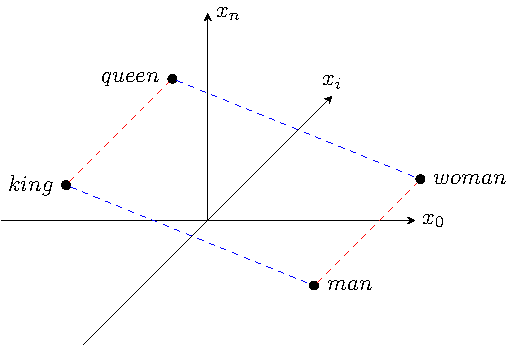
\includegraphics[width=0.7\textwidth]{../images/wordembedding} % 请确保图片路径正确
    \caption{词向量的正则性示例}
    \label{fig:word_embedding}
\end{figure}

最为著名的例子是“男人”、“女人”、“国王”和“王后”之间的关系(图 \ref{fig:word_embedding})。让我们对其稍作解析。图中揭示了两组平行关系,形成一个几何上的平行四边形:
\begin{itemize}
    \item \textbf{性别维度}:$\vec{国王} - \vec{男人} \approx \vec{女王} - \vec{女人}$
    \item \textbf{王权维度}:$\vec{国王} - \vec{女王} \approx \vec{男人} - \vec{女人}$
\end{itemize}
这个几何结构的核心在于,我们可以将语义关系看作是作用于语义概念的“算子”或“移动”。例如,从“男人”到“女王”,可以通过两条不同的路径到达:
\begin{enumerate}
    \item \texttt{男人} $\xrightarrow{+\text{王权移动}}$ \texttt{国王} $\xrightarrow{-\text{性别移动}}$ \texttt{女王}
    \item \texttt{男人} $\xrightarrow{-\text{性别移动}}$ \texttt{女人} $\xrightarrow{+\text{王权移动}}$ \texttt{女王}
\end{enumerate}
这两条路径的等价性,本质上反映了这些语义关系算子满足**交换律**:
\[
\text{“王权移动”} + \text{“性别移动”} = \text{“性别移动”} + \text{“王权移动”}
\]
这个在词嵌入中自然涌现的交换性,成为了我思考的起点:如果我们把这种关系正则性强制要求下来,去审视数学中最基础的算术运算,会发生什么呢?

\section{数字的双曲表示}
\label{sec:hyperbolic_representation}

2015 年的秋天,我拿数字和数字的运算关系做了一些实验。我考察了最简单的两个算术关系:“$+1$”(加一)和“$\times 2$”(乘二)。

此时,所有的数字都映射为空间的点,而“$+1$”和“$\times 2$”运算关系则映射为空间中的向量或变换。假设从任意一个数字 $\alpha$ 出发,我们可以进行一系列的运算关系组合,例如:
\begin{itemize}
    \item \textbf{路径1 (先加后乘)}:$(\alpha + 1) \times 2 = 2\alpha + 2$
    \item \textbf{路径2 (先乘后加)}:$(\alpha \times 2) + 1 = 2\alpha + 1$
\end{itemize}
我们立刻发现,无论起点 $\alpha$ 为何,这两个运算关系都**不具备交换性**。它们无法像词向量的语义关系那样形成一个闭合的平行四边形。

\begin{figure}[ht]
    \centering
    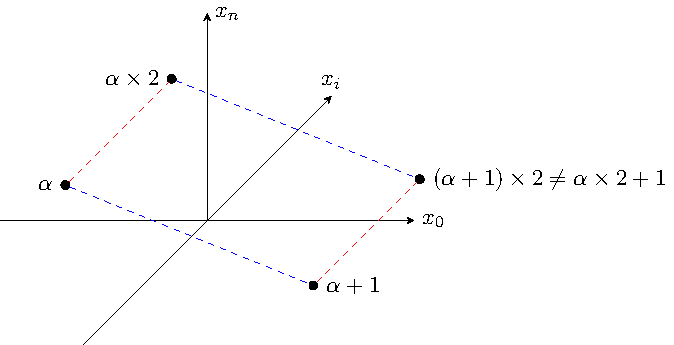
\includegraphics[width=0.6\textwidth]{../images/numberembedding} % 请确保图片路径正确
    \caption{数字嵌入中,加法与乘法运算的非交换性}
    \label{fig:number_embedding}
\end{figure}

平行四边形的缺失,意味着我们无法通过路径等价来约化操作序列,这将导致运算关系组合的**组合爆炸**(combinatorial explosion)无法避免。如果每个不同的表达式都需要在表征空间里占据一个唯一的、有限大的区域,那么随着表达式数量的指数级增长,任何一个体积呈多项式增长的空间(如欧几里得空间)都将很快被耗尽。

幸运的是,几何学里有一种空间,它的容量恰好是指数增长的,并且其内在几何(不存在全局的平行线)也与这种非交换性天然契合——这就是**双曲空间**。我决定拿双曲空间来尝试解决这个问题。\footnote{所有关系运算的可能组合的数量是一种复杂性度量。于是整个讨论隐含了体积或者面积正比于这个度量。这个观点在后续章节中还会有所阐发。}

经过一些尝试,我发现一种称之为“四阶无限边形铺嵌”的结构可以用来编码数字的加法和乘法。如图 \ref{fig:assignment2},在庞加莱圆盘模型中,我们可以构建一个高度对称的网格,其中一个方向的测地线族代表“$+1$”的关系,而与之正交的测地线族代表“$\times 2$”的关系。

\begin{figure}[ht]
    \centering
    \resizebox{0.5\textwidth}{!}{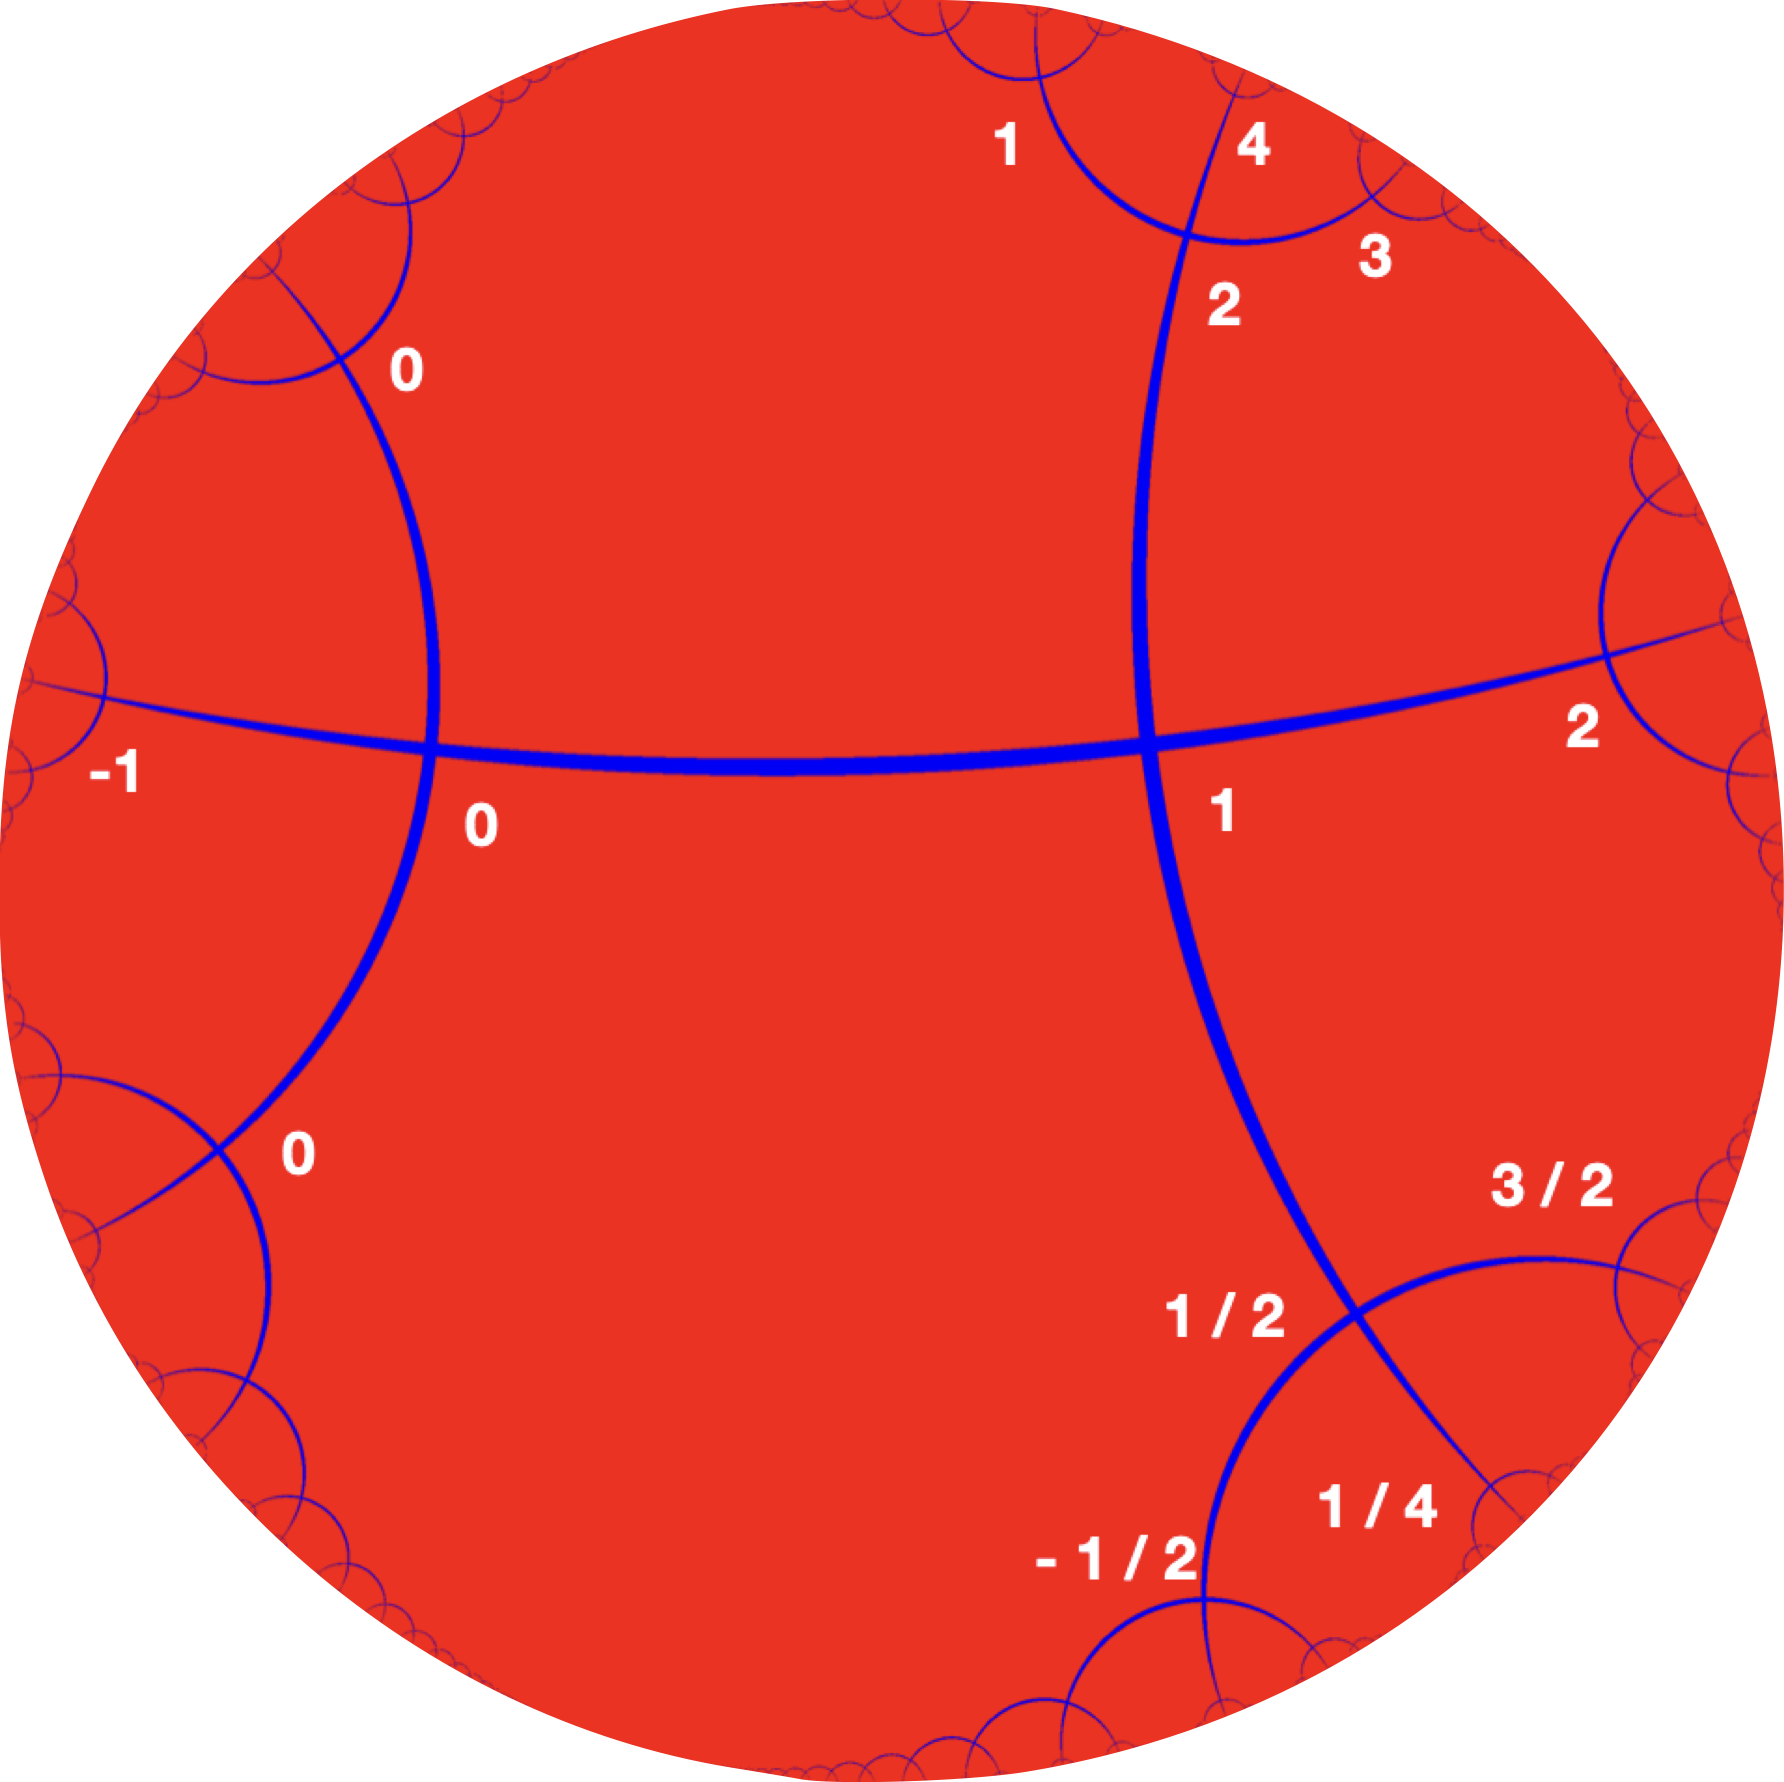
\includegraphics{../images/assignment2}} % 请确保图片路径正确
    \caption{庞加莱圆盘上的加乘关系与数字排布}
    \label{fig:assignment2}
\end{figure}

望着这些高度对称分布的离散点值,一个非常自然的问题产生了:这些离散的点值,能否被一个定义在整个庞加莱圆盘上的**连续函数**所描述?如果可以,那么我们就能将算术运算从离散的整数域,推广到连续的实数域,并为其建立一个真正的几何模型。

\section{流方程的引入}
\label{sec:flow_equation_intro}

时间飞逝到了 2019 年,我在一次出差的飞机上,突然想到既然我希望这些点值能够连续地分布,那么为何不直接从一个无穷小的生成过程出发呢?我在飞机上快速做了一些推导,结果是极为鼓舞的。几天之内,我就得到了一个描述加法与乘法双生成元无穷小过程的微分方程。

假设在我们的几何空间中,存在一个标量场 $a$(我们称之为**赋值场**),其值对应于数字。我们考察一个从赋值为 $a_0$ 的点出发,沿着一个方向走一小段距离 $\epsilon$ 的过程。设此方向与“纯加法”方向的夹角为 $\theta$。那么,无穷小的加法贡献为 $\mu \epsilon \cos \theta$,而无穷小的乘法贡献为 $e^{\lambda \epsilon \sin \theta}$(其中 $\mu$ 和 $\lambda$ 分别是加法和乘法生成元的强度)。

我们考虑两种等价的组合顺序:
\begin{itemize}
    \item \textbf{优先加法}:$a_{\epsilon} = (a_0 + \mu \epsilon \cos \theta)e^{\lambda \epsilon \sin \theta}$
    \item \textbf{优先乘法}:$a_{\epsilon} = a_0 e^{\lambda \epsilon \sin \theta} + \mu \epsilon \cos \theta$
\end{itemize}
对 $e^{\lambda \epsilon \sin \theta}$ 进行泰勒展开至一阶项 $1 + \lambda \epsilon \sin \theta$,并略去 $\epsilon^2$ 的高阶小项,两种情形都可以简化为同一个结果:
\[ a_{\epsilon} \approx a_0 + \epsilon (a_0 \lambda \sin \theta + \mu \cos \theta) \]
令 $da = a_{\epsilon} - a_0$ 且 $ds = \epsilon$,在取极限 $\epsilon \to 0$ 时,我们便得到了如下的微分方程:
\begin{equation}
    \frac{da}{ds} = \mu \cos \theta + a \lambda \sin \theta
    \label{eq:flow_equation_derivation}
\end{equation}
整个推导非常初等,但其意义重大。因为它刻画了一个计算的“流动”过程,我称之为“**流方程**”(Flow Equation)。这个方程是可解的,并且其解自然地兼容了离散的生成过程。流方程成为了连接离散算术操作与连续几何空间的桥梁。

\section{第一个解析解}
\label{sec:first_analytical_solution}

2021 年春天,在公司的支持下,我与两位实习生开始了更为严谨的研究。来自山东大学的张乐同学利用分离变量法,很快推导出了流方程的一个解析解。我们发现,在上半平面模型 ($\mathbb{H}^2 = \{(x, y) \in \mathbb{R}^2 \mid y > 0\}$) 中,赋值场 $a$ 的一个优雅解是:
\begin{equation}
    a(x, y) = - \frac{x}{y}
    \label{eq:first_solution}
\end{equation}
并且,只要我们适当地调整空间的度规,这个解对于任意的生成元强度 $\mu$ 和 $\lambda$ 都成立。

这个解析解的获得,是我们研究的第一个里程碑。在此之前,我们仅有离散的结构和模糊的猜想;而现在,我们拥有了第一个可以被精确分析和研究的、严格的数学对象。我将其可视化,得到了一个由彼此正交的测地线和伪圆构成的网格(图 \ref{fig:assignment1})。

\begin{figure}[ht]
    \centering
    \resizebox{0.8\textwidth}{!}{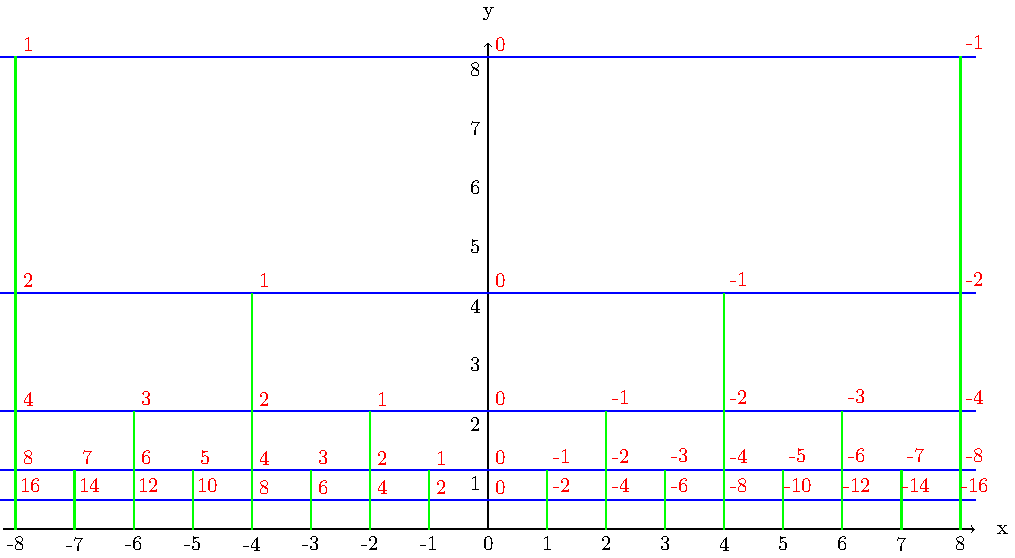
\includegraphics{../images/01-grid-example-1}} % 请确保图片路径正确
    \caption{上半平面模型中的加乘网格与赋值 $a = -x/y$}
    \label{fig:assignment1}
\end{figure}

在这个网格上,我们可以清晰地看到算术运算的几何路径。例如,图 \ref{fig:encoding} 中展示了三条不同的路径,它们都从赋值为 $1$ 的点出发,最终到达赋值为 $3$ 的点,分别编码了三种代数上等价的算术表达式:
\begin{itemize}
    \item \textbf{黑色路径}: $1 \times 8 - 5 = 3$
    \item \textbf{紫红色路径}: $(1 - \frac{5}{8}) \times 8 = 3$
    \item \textbf{褐色路径}: $(((1 - \frac{1}{8}) \times 2 - \frac{2}{4}) \times 2 - 1) \times 2 = 3$
\end{itemize}

\begin{figure}[ht]
    \centering
    \resizebox{0.8\textwidth}{!}{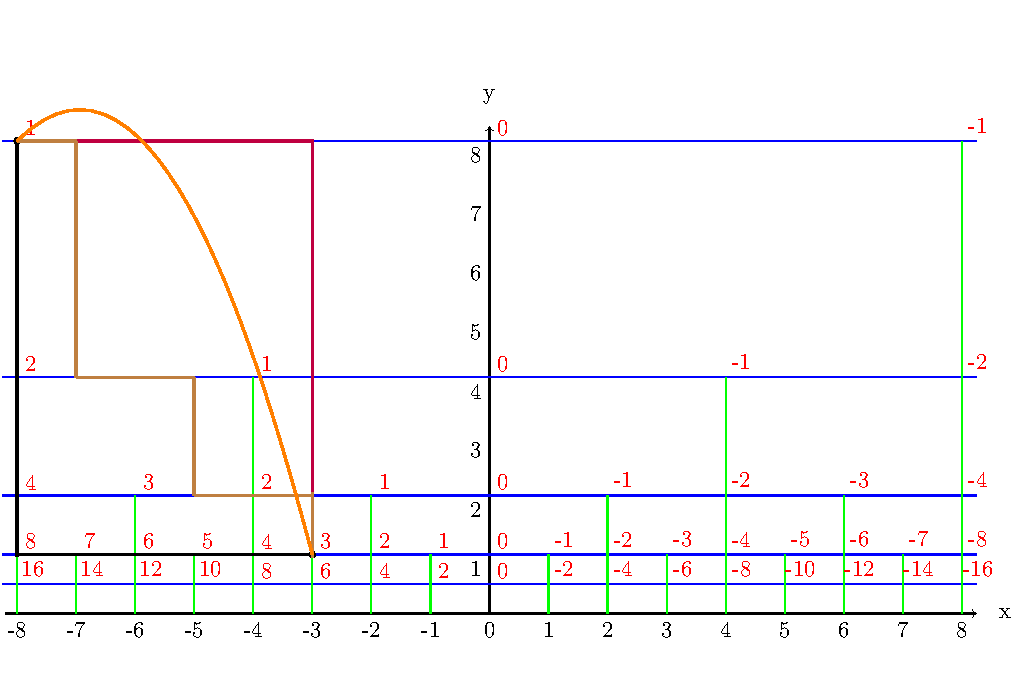
\includegraphics{../images/encoding}} % 请确保图片路径正确
    \caption{不同路径编码等价的算术表达式}
    \label{fig:encoding}
\end{figure}

这些离散路径的存在,以及它们之间的代数等价关系,引出了一系列深刻的问题:这些路径的几何性质有何不同?我们如何量化它们之间的差异?更进一步,图中的橙色平滑曲线又编码了什么?它似乎代表了一种同时累积加法小量和乘法小量的、非传统的积分过程。

这些问题,正是我们将在后续章节中,通过引入“算术挠率”、“累积交换空间”等核心概念来逐步解答的。这第一个解析解,为我们打开了通往算术表达式几何宏伟殿堂的大门。
\newpage

% !TEX root = ../main.tex
% ----------------------------------------------------------------
% Chapter 2: 算术表达式的语言 (The Language of Arithmetic Expressions)
% ----------------------------------------------------------------

\chapter{算术表达式的语言}
\label{chap:language_of_aeg}

在第一章中,我们通过一段探索性的历史回顾,初步认识了算术表达式几何的起源和核心思想。我们看到,简单的算术运算背后可能隐藏着深刻的几何结构,而“流方程”则为连接离散操作与连续空间提供了可能。

为了深入探索这片海域,我们必须首先打磨我们的航海工具——也就是为“算术表达式”本身建立一套精确、严谨的语言。本章将致力于此,我们将从最基础的定义出发,逐步引入可线索化表达式、路径表示法,并最终触及所有算术过程的代数源头——自由群 $F_2$。

\section{算术表达式及其树结构}
\label{sec:arithmetic_expression}

从计算机科学的角度来看,算术表达式是一种抽象的递归数据类型。它有两种等价的表示形式:我们日常书写的**字串表示**,以及其内在逻辑结构的**树表示**。例如,对于表达式:
\begin{equation}
    (((((1 \times 2) \times 2) - 1) \times (2 + 1)) - 6)
\end{equation}
其对应的解析树如图 \ref{fig:syntaxtree_ch2} 所示。树的叶子节点是操作数(数字),内部节点是操作符。

\begin{figure}[ht]
    \centering
    \resizebox{0.3\textwidth}{!}{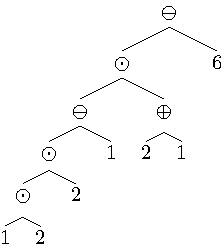
\includegraphics{../images/02-example-expression-syntax-tree.pdf}} % 请确保图片路径正确
    \caption{算术表达式的解析树表示}
    \label{fig:syntaxtree_ch2}
\end{figure}

为了严谨,我们首先在有理数域 $\mathbb{Q}$ 上给出一个生成式的递归定义。它指明:有理数本身是算术表达式;而算术表达式通过四则运算的组合,仍然构成算术表达式。

\begin{definition}[算术表达式]
    \label{def:arithmetic_expression_formal}
    数域 $\mathbb{Q}$ 上的\textbf{算术表达式} $a$ 是被如下产生式规则(production rules)定义的结构:
    \begin{equation}
        \begin{aligned}
            a & \longleftarrow x \\
            a & \longleftarrow ( a + a ) \\
            a & \longleftarrow ( a - a ) \\
            a & \longleftarrow ( a \times a ) \\
            a & \longleftarrow ( a \div a )
        \end{aligned}
    \end{equation}
    其中 $x \in \mathbb{Q}$。所有这类表达式的集合记为 $\mathbb{E}[\mathbb{Q}]$。
\end{definition}

在这个递归结构上,我们可以递归地定义一个**求值**(evaluation)过程 $\nu(a)$,它将一个表达式映射到一个有理数值。

\begin{definition}[求值函数 $\nu$]
    \label{def:evaluation_nu}
    求值函数 $\nu: \mathbb{E}[\mathbb{Q}] \to \mathbb{Q}$ 是一个部分函数(partial function),其定义如下:
    \begin{itemize}
        \item \textbf{常数叶节点}: 对任意 $x \in \mathbb{Q}$, $\nu(x) = x$。
        \item \textbf{加法节点}: 对任意 $(a+b) \in \mathbb{E}[\mathbb{Q}]$, $\nu((a + b)) = \nu(a) + \nu(b)$。
        \item \textbf{减法节点}: 对任意 $(a-b) \in \mathbb{E}[\mathbb{Q}]$, $\nu((a - b)) = \nu(a) - \nu(b)$。
        \item \textbf{乘法节点}: 对任意 $(a \times b) \in \mathbb{E}[\mathbb{Q}]$, $\nu((a \times b)) = \nu(a) \nu(b)$。
        \item \textbf{除法节点}: 对任意 $(a \div b) \in \mathbb{E}[\mathbb{Q}]$,若 $\nu(b) \neq 0$,则 $\nu((a \div b)) = \nu(a) / \nu(b)$。
    \end{itemize}
    如果 $\nu(a)$ 有定义,我们称表达式 $a$ 是**可求值的**(evaluable)。
\end{definition}

值得注意的是,我们将表达式定义在有理数域 $\mathbb{Q}$ 上,而非更熟悉的实数域 $\mathbb{R}$。这是为了回避一个深刻的理论困难:在 $\mathbb{R}$ 上,一个任意给定的算术表达式的值是否为零是不可判定的\footnote{这与 Richardson 定理相关。该定理表明,包含特定函数(如 $\pi, \ln 2, e^x, \sin x$)的实数表达式的“零点问题”是不可判定的。}。由于除法操作要求除数不为零,若定义在 $\mathbb{R}$ 上,我们将无法从纯粹的语法层面保证一个表达式是可求值的(即语义上有效)。从 $\mathbb{Q}$ 出发,我们可以在一个坚实的基础上构建理论,未来再通过完备化的方法将其推广到 $\mathbb{R}$。这揭示了**语法**(表达式的结构)与**语义**(表达式的值)之间的重要区别,而除零错误,正是在几何与函数论的观点下,体现为我们理论中的**奇点**(singularity)。

\section{可线索化表达式与典范式}
\label{sec:threadlike_expressions}

对于一个普通的表达式树,其内部节点的求值顺序通常不唯一。但有一些特殊的表达式,它们的求值顺序是唯一的,这对我们将表达式理解为一条“路径”至关重要。

\begin{definition}[可线索化表达式]
    \label{def:threadlike_expression}
    一个**可线索化表达式**(threadlike expression)是指其树表示中,所有的左子节点(或所有右子节点)均为叶节点(操作数)的表达式。
\end{definition}

\begin{figure}[ht]
    \centering
    \resizebox{0.8\textwidth}{!}{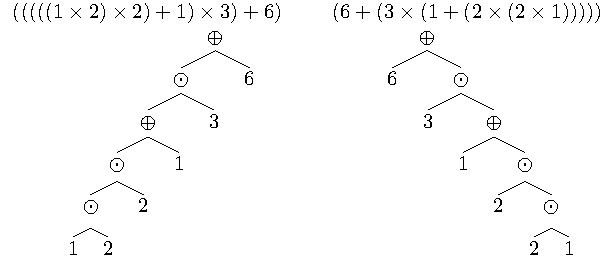
\includegraphics{../images/03-example-expression-syntax-tree-left-right.pdf}} % 请确保图片路径正确
    \caption{向右展开(左)与向左展开(右)的可线索化表达式}
    \label{fig:threadlike_trees}
\end{figure}

如图 \ref{fig:threadlike_trees} 所示,这类表达式的结构形如一条“主干”不断延伸,因此其求值顺序是唯一确定的。向左或向右展开完全是对称的,为方便起见,我们通常选取一种作为标准形式。可线索化表达式构成了我们理论中“路径”的原型。

更进一步,我们可以定义一种规范形式。

\begin{definition}[交错式典范式]
    \label{def:alternating_canonical_form}
    一个**交错式可线索化表达式**(alternating threadlike expression)是指其中加法类运算(加、减)与乘法类运算(乘、除)交替出现的可线索化表达式。
\end{definition}

任何一个可线索化表达式,都可以通过适当地添加“$+0$”项或“$\times 1$”项来补足成为一个交错式。因此,交错式可以被视为可线索化表达式的一种**典范形式**(canonical form)。

\section{路径与柯里化表示}
\label{sec:path_and_currying}

为了更方便地处理可线索化表达式的动态、序列化特性,我们引入一种源自函数式编程的**柯里化**(Currying)表示法。它将一个表达式看作是一系列单参数算子(operator)的依次作用。

\begin{definition}[基本算术算子]
    \label{def:arithmetic_operators}
    我们定义如下四种基本算术算子:
    \begin{itemize}
        \item \textbf{加法算子}: $\oplus_\mu: x \mapsto x + \mu$
        \item \textbf{减法算子}: $\ominus_\mu: x \mapsto x - \mu$
        \item \textbf{乘法算子}: $\otimes_\lambda: x \mapsto x \cdot e^\lambda$
        \item \textbf{除法算子}: $\oslash_\lambda: x \mapsto x \cdot e^{-\lambda}$
    \end{itemize}
    这里,我们将乘法因子参数化为对数形式 $e^\lambda$,使得乘法在参数层面也具有加法结构。这对于后续理论的统一至关重要。
\end{definition}

借助这些算子,一个可线索化表达式,例如 $((((x_0 + \mu_1) \cdot e^{\lambda_1}) + \mu_2) \cdot e^{\lambda_2})$,可以被看作是算子序列 $(\oplus_{\mu_1}, \otimes_{\lambda_1}, \oplus_{\mu_2}, \otimes_{\lambda_2})$ 作用在初始值 $x_0$ 上的过程。这启发我们引入一种简洁的**路径记法**。

\begin{definition}[路径记法]
    \label{def:path_notation}
    对于一个算子序列 $\gamma = (o_1, o_2, \dots, o_n)$,它作用于初始值 $x$ 的过程记为:
    \[ x \cdot \gamma \quad \text{或} \quad x \, o_1 o_2 \dots o_n \coloneqq o_n(o_{n-1}(\dots(o_1(x))\dots)) \]
    我们称 $\gamma$ 为一条**自由路径**(free path),它是一个函数。而 $x \cdot \gamma$ 称为一条**约束路径**(bounded path),其结果是一个值。
\end{definition}

例如,表达式 $((((1 \times 2) + 3) \times 4) + 5)$ 可以被写成约束路径:
$1 \cdot \otimes_{\ln 2} \oplus_3 \otimes_{\ln 4} \oplus_5$。

这种路径表示法有一个非常重要的性质:算子复合满足结合律。

\begin{lemma}[路径的结合律]
    \label{lemma:path_associativity}
    对于任意算子 $a, b, c$,路径复合满足结合律,即:$(a \cdot b) \cdot c = a \cdot (b \cdot c)$。
\end{lemma}
\begin{proof}
    设算子 $a, b, c$ 对应的函数分别为 $\mathbf{a}, \mathbf{b}, \mathbf{c}$。根据函数复合的定义,路径记法 $a \cdot b$ 对应的函数是 $\mathbf{b} \circ \mathbf{a}$。
    因此,$(a \cdot b) \cdot c$ 对应的函数为 $\mathbf{c} \circ (\mathbf{b} \circ \mathbf{a})$。
    而 $a \cdot (b \cdot c)$ 对应的函数为 $(\mathbf{c} \circ \mathbf{b}) \circ \mathbf{a}$。
    由于函数复合本身满足结合律,即 $\mathbf{c} \circ (\mathbf{b} \circ \mathbf{a}) = (\mathbf{c} \circ \mathbf{b}) \circ \mathbf{a}$,故引理得证。
\end{proof}
路径的结合律是我们能够将算术表达式视为几何空间中良定义“路径”的代数基础。

\section{作为运算源头的自由群 $F_2$}
\label{sec:free_group_f2}

现在,让我们从更抽象的层面审视这些算术路径的起源。我们将具体的加法和乘法操作,抽象为两个生成元:
\begin{itemize}
    \item $\mathbf{x}$: 代表一次抽象的“加性”操作(如 $\oplus_{\mu_0}$)。
    \item $\mathbf{y}$: 代表一次抽象的“乘性”操作(如 $\otimes_{\lambda_0}$)。
\end{itemize}
所有可能的操作序列,包括它们各自的逆操作($\mathbf{x}^{-1}$ 代表减法,$\mathbf{y}^{-1}$ 代表除法),构成了一个代数结构。这个结构中,除了 $g \cdot g^{-1} = \text{id}$ 之外,没有任何其他运算关系。这正是**自由群**(free group)的定义。

\begin{definition}[算术操作的自由群]
    \label{def:free_group_F2}
    所有抽象算术路径的集合,在路径拼接操作下,构成了由两个生成元 $\mathbf{x}$ 和 $\mathbf{y}$ 生成的**自由群 $F_2 = \langle \mathbf{x}, \mathbf{y} \rangle$**。
\end{definition}

将 $F_2$ 视为我们理论的起点,具有极其重要的意义。$F_2$ 中的每一个元素(一个“词”,word)都唯一地对应着一条特定的、无任何化简的操作序列。它是一个“绝对自由”的、纯粹符号化的宇宙,其中充满了无限多条形态各异的路径。

在这个意义上,**$F_2$ 是所有算术复杂性的“始祖”或“本源”**。我们后续研究的所有具体的、具有特定几何结构的算术表达式空间(如 $\mathfrak{E}_0, \mathfrak{E}_1$),都可以被看作是在 $F_2$ 这个无限的、纯粹时间性的序列之海中,通过施加特定的“关系”(relations)或“等价”,从而“凝聚”(condense)而成的、具有空间结构的产物。

本章我们建立了算术表达式的语言体系,从具象的表达式,到抽象的自由群。下一章,我们将探讨这些表达式作为动态过程的核心规律——流方程。\newpage
% !TEX root = ../main.tex
% ----------------------------------------------------------------
% Chapter 3: 流方程:算术的动力学 (The Flow Equation: Dynamics of Arithmetic)
% ----------------------------------------------------------------

\chapter{流方程:算术的动力学}
\label{chap:flow_equation}

在第二章中,我们为算术表达式建立了严谨的代数语言,从具体的表达式树,到序列化的路径表示,最终追溯到其代数源头——自由群 $F_2$。这个语言体系为我们描述算术的“静态结构”提供了基础。

然而,算术的本质是动态的,它是一个生成与演化的过程。为了捕捉这一动态特性,我们需要一套“运动定律”。本章将详细阐述这套定律的核心——**流方程**(Flow Equation)。我们将展示,这个简洁的微分方程如何从最基本的无穷小生成过程出发,统一地描述了算术值在几何空间中的演化,并揭示了其背后深刻的数学与物理内涵。

\section{从无穷小过程推导}
\label{sec:derivation_of_flow_equation}

让我们重返第一章结尾提出的问题:如何将离散的算术操作连续化?答案在于考察一个无穷小的生成过程。

设想我们在一个几何空间中,其上定义了一个赋值场 $a$。我们从空间中赋值为 $a_0$ 的一点出发,沿着一个方向进行一段无穷小的移动,路径长度为 $ds$。我们将这个移动分解为“纯加法”和“纯乘法”两个正交的分量。设移动方向与“纯加法”主轴方向的夹角为 $\theta$,并令 $(\mu, \lambda)$ 为描述加法与乘法强度的**算术基因**(arithmetic gene)。
\begin{itemize}
    \item 移动在加法主轴上的投影长度为 $ds \cos\theta$,产生的加法贡献为 $\mu (ds \cos\theta)$。
    \item 移动在乘法主轴上的投影长度为 $ds \sin\theta$,产生的乘法贡献因子为 $e^{\lambda (ds \sin\theta)}$。
\end{itemize}
在无穷小尺度下,这两个操作的先后顺序不影响最终结果。我们以前馈路径为例,新的赋值 $a(s_0+ds)$ 为:
\[
a(s_0+ds) = \left( a(s_0) + \mu ds \cos\theta \right) e^{\lambda ds \sin\theta}
\]
对指数项进行一阶泰勒展开,$e^x \approx 1+x$(因为 $ds$ 是无穷小量,$(ds)^2$ 及更高阶项可以忽略),我们得到:
\begin{align*}
    a(s_0+ds) &\approx (a_0 + \mu ds \cos\theta)(1 + \lambda ds \sin\theta) \\
    &\approx a_0 + a_0 \lambda ds \sin\theta + \mu ds \cos\theta + \mu\lambda (ds)^2 \cos\theta \sin\theta \\
    &\approx a_0 + ds( \mu \cos\theta + a_0 \lambda \sin\theta )
\end{align*}
整理后可得:
\[
\frac{a(s_0+ds) - a_0}{ds} = \mu \cos\theta + a_0 \lambda \sin\theta
\]
取极限 $ds \to 0$,我们就得到了描述赋值 $a$ 沿着路径 $s$ 变化规律的微分方程。

\begin{definition}[流方程]
    \label{def:flow_equation}
    在算术表达式几何中,描述赋值 $a$ 随路径参数 $s$ 变化的**流方程**(Flow Equation)定义为:
    \begin{equation}
        \frac{da}{ds} = \mu \cos\theta + a \lambda \sin\theta
        \label{eq:flow_equation}
    \end{equation}
    其中 $(\mu, \lambda)$ 为算术基因,$\theta$ 为路径方向与加法主轴的夹角。
\end{definition}

流方程是 AEG 的动力学核心。它表明,赋值 $a$ 的变化率由两部分驱动:一部分是与当前值无关的**加性驱动**($\mu \cos\theta$),另一部分是与当前值 $a$ 成正比的**乘性驱动**($a \lambda \sin\theta$)。

\section{形式解及其群性质}
\label{sec:formal_solution}

流方程 (\ref{eq:flow_equation}) 是一个一阶线性常微分方程,对于固定的方向 $\theta$,它是可解的。

\begin{proposition}[流方程的形式解]
    \label{prop:formal_solution}
    对于给定的初始条件 $a(s=0)=a_0$,以及恒定的方向 $\theta \neq k\pi$ ($k \in \mathbb{Z}$),流方程 (\ref{eq:flow_equation}) 的解为:
    \begin{equation}
        a(s) = \left(a_0 + \frac{\mu}{\lambda} \cot\theta\right) e^{\lambda s \sin\theta} - \frac{\mu}{\lambda} \cot\theta
        \label{eq:formal_solution}
    \end{equation}
\end{proposition}
\begin{proof}
    方程 (\ref{eq:flow_equation}) 可写为 $\frac{da}{a\lambda\sin\theta + \mu\cos\theta} = ds$。
    对两边积分:
    \[ \int \frac{da}{a\lambda\sin\theta + \mu\cos\theta} = \int ds \]
    \[ \frac{1}{\lambda\sin\theta} \ln|a\lambda\sin\theta + \mu\cos\theta| = s + C \]
    \[ a\lambda\sin\theta + \mu\cos\theta = e^{\lambda s \sin\theta + C'} = C_0 e^{\lambda s \sin\theta} \]
    代入初始条件 $a(0)=a_0$,可得 $C_0 = a_0\lambda\sin\theta + \mu\cos\theta$。
    代回并整理可得方程 (\ref{eq:formal_solution})。
\end{proof}

这个形式解不仅给出了赋值 $a$ 的演化轨迹,更重要的是,它揭示了在一个固定的方向上,“流动”操作具有良好的代数结构。

\begin{proposition}[流动的单参数群性质]
    \label{prop:one_parameter_group}
    对于任意固定的方向 $\theta$,由形式解 (\ref{eq:formal_solution}) 定义的变换 $T_s: a_0 \mapsto a(s)$ 构成一个以路径长度 $s$ 为参数的单参数变换群。
\end{proposition}
\begin{proof}
    我们需要验证群的三个公理:
    \begin{enumerate}
        \item \textbf{封闭性(变换合成)}:$T_{s_2}(T_{s_1}(a_0)) = T_{s_1+s_2}(a_0)$。
        令 $a_1 = T_{s_1}(a_0)$。则 $a_1 + \frac{\mu}{\lambda}\cot\theta = (a_0 + \frac{\mu}{\lambda}\cot\theta)e^{\lambda s_1 \sin\theta}$。
        $T_{s_2}(a_1) = (a_1 + \frac{\mu}{\lambda}\cot\theta)e^{\lambda s_2 \sin\theta} - \frac{\mu}{\lambda}\cot\theta = (a_0 + \frac{\mu}{\lambda}\cot\theta)e^{\lambda s_1 \sin\theta}e^{\lambda s_2 \sin\theta} - \frac{\mu}{\lambda}\cot\theta = (a_0 + \frac{\mu}{\lambda}\cot\theta)e^{\lambda (s_1+s_2) \sin\theta} - \frac{\mu}{\lambda}\cot\theta = T_{s_1+s_2}(a_0)$。
        \item \textbf{单位元}:$T_0(a_0) = a_0$。
        当 $s=0$,$a(0) = (a_0 + \frac{\mu}{\lambda}\cot\theta)e^0 - \frac{\mu}{\lambda}\cot\theta = a_0$。
        \item \textbf{逆元}:$T_{-s}(T_s(a_0)) = a_0$。
        根据封闭性,$T_{-s}(T_s(a_0)) = T_{s-s}(a_0) = T_0(a_0) = a_0$。
    \end{enumerate}
    所有公理均满足,故命题成立。
\end{proof}
这个群性质意义重大,它保证了在 AEG 空间中沿直线路径的“流动”是一种自洽、可逆、可叠加的变换,为将路径积分为良定义的几何对象提供了代数基础。

\section{程函方程与波前传播}
\label{sec:eikonal_equation}

流方程 (\ref{eq:flow_equation}) 描述了赋值 $a$ 沿任意方向 $\theta$ 的变化。一个自然的问题是:$a$ 变化最快的方向在哪里?其变化率的幅值是多少?这引导我们将流方程改写为一种坐标无关的形式。

首先,我们寻找 $a$ 值保持不变的方向,即等值线(contour line)方向 $\theta_c$,此时 $\frac{da}{ds}=0$:
\[ \mu\cos\theta_c + a\lambda\sin\theta_c = 0 \implies \tan\theta_c = -\frac{\mu}{a\lambda} \]
梯度(gradient)方向 $\theta_g$ 与等值线方向正交,即 $\theta_g = \theta_c \pm \frac{\pi}{2}$。沿梯度方向,$a$ 的变化率达到最大值。将 $\theta_g$ 代入流方程:
\begin{align*}
    \left. \frac{da}{ds} \right|_{\theta_g} &= \mu\cos(\theta_c \pm \frac{\pi}{2}) + a\lambda\sin(\theta_c \pm \frac{\pi}{2}) \\
    &= \mu(\mp\sin\theta_c) + a\lambda(\pm\cos\theta_c) \\
    &= \pm (\mu(-\sin\theta_c) + a\lambda\cos\theta_c)
\end{align*}
从 $\tan\theta_c = -{\mu}/{a\lambda}$ 可构建一个直角三角形,其对边为 $\mu$,邻边为 $-a\lambda$(或反之),斜边为 $\sqrt{\mu^2 + (a\lambda)^2}$。由此可得 $\sin\theta_c = \frac{\mu}{\pm\sqrt{\mu^2+(a\lambda)^2}}$ 和 $\cos\theta_c = \frac{-a\lambda}{\pm\sqrt{\mu^2+(a\lambda)^2}}$。代入上式:
\[
\left. \frac{da}{ds} \right|_{\theta_g} = \pm \left( \mu\left(-\frac{\mu}{\pm\sqrt{\dots}}\right) + a\lambda\left(\frac{-a\lambda}{\pm\sqrt{\dots}}\right) \right) = \pm \frac{-(\mu^2 + (a\lambda)^2)}{\pm\sqrt{\mu^2+(a\lambda)^2}}
\]
其幅值为 $||\nabla a|| = \left| \left. \frac{da}{ds} \right|_{\theta_g} \right| = \sqrt{\mu^2 + (a\lambda)^2}$。

\begin{theorem}[流方程的程函形式]
    \label{thm:eikonal_form}
    流方程 (\ref{eq:flow_equation}) 的坐标无关形式为:
    \begin{equation}
        ||\nabla a|| = \sqrt{\mu^2 + a^2\lambda^2}
        \label{eq:eikonal_equation}
    \end{equation}
    这是一个**程函方程**(Eikonal Equation)。
\end{theorem}

将流方程表述为程函方程,是 AEG 理论与物理学和经典力学建立深刻联系的关键一步。
\begin{itemize}
    \item 在**物理光学**中,程函方程描述了波前(wavefront)的传播。因此,我们可以将赋值场 $a$ 的演化,直观地想象为一种信息或“波前”在几何空间中的传播过程。
    \item 在**经典力学**中,程函方程是哈密顿-雅可比方程(Hamilton-Jacobi equation)的一种特例。这暗示了 AEG 框架可能具有更深层的拉格朗日/哈密顿力学结构,其中赋值 $a$ 扮演了作用量的角色。
\end{itemize}
这个联系极大地丰富了 AEG 的内涵,允许我们借鉴和运用来自其他物理领域的强大分析工具和深刻的直觉。

\section{连续与离散生成的兼容性}
\label{sec:consistency}

我们在第二章定义了离散的算术算子(如 $\oplus_\mu, \otimes_\lambda$),在本章推导了描述连续流动的流方程。一个至关重要的问题是:这两套描述体系是否兼容?流方程的解,在特定方向上,是否能精确地还原离散的算术操作?

答案是肯定的。我们从流方程的形式解 (\ref{eq:formal_solution}) 出发,将其在 $\theta$ 取 $\frac{\pi}{2}$ 的倍数时进行考察。
\[ a(s) = a_0 e^{\lambda s \sin \theta} + \frac{\mu}{\lambda} (e^{\lambda s \sin \theta} - 1) \cot \theta \]
\begin{itemize}
    \item \textbf{纯加法方向 ($\theta=0$)}: $\sin\theta=0, \cos\theta=1$。此时形式解不适用,需回到原方程 $\frac{da}{ds} = \mu$,直接积分得 $a(s) = a_0 + \mu s$。这精确对应了离散算子 $\oplus_\mu$ 的累次作用。
    \item \textbf{纯乘法方向 ($\theta=\pi/2$)}: $\sin\theta=1, \cos\theta=0$。此时 $\cot\theta=0$,形式解变为 $a(s) = a_0 e^{\lambda s}$。这精确对应了离散算子 $\otimes_\lambda$ 的累次作用。
    \item \textbf{纯减法方向 ($\theta=\pi$)}: $\sin\theta=0, \cos\theta=-1$。原方程为 $\frac{da}{ds} = -\mu$,积分得 $a(s) = a_0 - \mu s$。
    \item \textbf{纯除法方向 ($\theta=3\pi/2$)}: $\sin\theta=-1, \cos\theta=0$。形式解变为 $a(s) = a_0 e^{-\lambda s}$。
\end{itemize}

这一结果有力地证明了,由无穷小过程推导出的连续流方程,是第二章中定义的离散自由生成群在几何上的自然延伸。流方程的解在主轴方向上精确地退化为离散的算术生成规则,这表明我们的理论框架是**自洽的**。连续的“流动”与离散的“跳跃”在 AEG 的世界里得到了和谐的统一。

% ----------------------------------------------------------------
% Chapter 4: 算术挠率与累积交换空间 (Arithmetic Torsion and the Accumulative Commutative Space)
% ----------------------------------------------------------------

\chapter{算术挠率与累积交换空间}
\label{chap:torsion_and_acs}

在第三章中,我们建立了算术表达式几何的动力学核心——流方程。它描述了赋值 $a$ 如何沿着一条给定的几何路径进行演化。然而,正如我们在第一章的例子中所见,连接相同起点和终点的不同路径,其代数表达式往往不等价。算术运算的非交换性,尤其是加法与乘法的混合,导致了计算结果的路径依赖性。

这一章的目标,就是引入一个核心概念来精确地量化这种路径依赖效应,我们称之为**算术挠率**(Arithmetic Torsion)。为了测量这个量,我们必须构建一个特殊的几何舞台,即**累积交换空间**(Accumulative Commutative Space, ACS)。最终,我们将建立一个连接代数计算与几何测度的“三重恒等式”,它构成了我们理论的基石之一。

\section{局部挠率与交换性的失效:代数的裂痕}
\label{sec:local_torsion}

我们从最简单的非交换操作对开始:一次加法和一次乘法。考虑从同一个初始值 $x_0$ 出发的两条不同路径:
\begin{itemize}
    \item \textbf{路径1}(先加后乘):$x_0 \cdot \oplus_\mu \otimes_\lambda$,其值为 $(x_0+\mu)e^\lambda$。
    \item \textbf{路径2}(先乘后加):$x_0 \cdot \otimes_\lambda \oplus_\mu$,其值为 $x_0 e^\lambda + \mu$。
\end{itemize}
显然,这两条路径的终点值是不同的。它们的差值,揭示了算术运算在局部层面的非交换性。

\begin{definition}[局部算术挠率]
    \label{def:local_torsion}
    对于加法算子 $\oplus_\mu$ 和乘法算子 $\otimes_\lambda$,其**局部算术挠率**(local arithmetic torsion)$\tau_{\text{local}}$ 定义为:
    \begin{equation}
        \tau_{\text{local}} = \nu(x_0 \cdot \oplus_\mu \otimes_\lambda) - \nu(x_0 \cdot \otimes_\lambda \oplus_\mu)
        \label{eq:local_torsion}
    \end{equation}
    计算可得:
    \[
        \tau_{\text{local}} = (x_0+\mu)e^\lambda - (x_0 e^\lambda + \mu) = x_0 e^\lambda + \mu e^\lambda - x_0 e^\lambda - \mu = \mu(e^\lambda - 1)
    \]
\end{definition}
一个关键的观察是,局部挠率 $\tau_{\text{local}}$ 是一个**常数**,它只依赖于算术基因 $(\mu, \lambda)$,而与初始值 $x_0$ 无关。

我们可以将这种局部非交换性带来的差异,形象地比喻为算术表达式空间中的一道“**代数裂痕**”(algebraic tear)。如图 \ref{fig:torsion_ch4} 所示,两条路径无法自然地形成一个闭合的回路,它们之间存在一个由挠率决定的“缺口”。这个固有的“开放”状态,正是非交换性的几何体现。

\begin{figure}[ht]
    \centering
    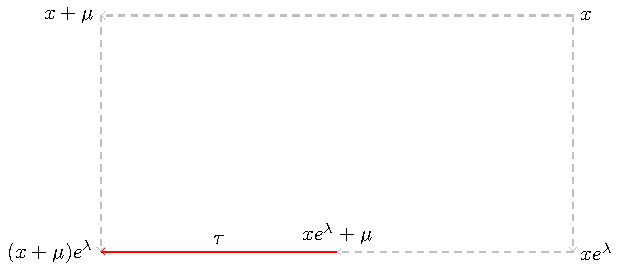
\includegraphics[width=0.7\textwidth]{../images/torsion} % 请确保图片路径正确
    \caption{局部挠率表现为几何路径上的“缺口”或“裂痕”}
    \label{fig:torsion_ch4}
\end{figure}

\section{交换画布的需求:ACS的引入}
\label{sec:introducing_acs}

既然局部的非交换性会产生“裂痕”,那么沿着一条由成百上千个操作组成的任意路径 $\gamma$,这些微小的裂痕将如何累积?我们又该如何测量这些累积效应的总和?

直接在表达式空间中进行测量是困难的,因为我们想要比较的两条路径(例如,一条路径和它的某种“逆路径”)通常不会形成一个闭合回路,这使得格林公式或斯托克斯定理等依赖于闭合边界的积分工具难以直接应用。

为了解决这个问题,我们需要构建一个新的参考空间,一个“**交换画布**”(commutative canvas)。在这个空间里,无论原始路径的非交换性有多复杂,我们关心的两条路径都能够共享相同的起点和终点,从而围成一个良定义的有界区域。这个特殊的参考空间,就是**累积交换空间**。

\begin{definition}[累积交换空间]
    \label{def:acs}
    **累积交换空间**(Accumulative Commutative Space, ACS),记为 $\mathcal{A}$,是一个二维欧几里得平面。对于任意一条算术路径 $\gamma$,其在 ACS 中的坐标 $(A_\gamma, M_\gamma)$ 由路径上所有操作的参数通过**交换性的累加**得到:
    \begin{itemize}
        \item \textbf{累积加性载荷 (Accumulated Additive Charge)}: $A_\gamma = \sum_k \mu_k$
        \item \textbf{累积乘性载荷 (Accumulated Multiplicative Charge)}: $M_\gamma = \sum_k \lambda_k$
    \end{itemize}
    其中 $\mu_k$ 是路径中第 $k$ 个加法类操作的参数,$\lambda_k$ 是第 $k$ 个乘法类操作的(对数)参数。
\end{definition}

ACS 的构造完全忽略了操作的顺序,只关心其“净含量”。它的关键特性在于:一条路径 $\gamma$ 和它的“反序路径” $\bar{\gamma}$(我们将在下一节精确定义),由于包含了完全相同的操作集合,它们在 ACS 中的起点(通常是原点 $(0,0)$)和**终点** $(A_\gamma, M_\gamma)$ 是**完全相同的**。

这样一来,尽管这两条路径在 ACS 中的轨迹可能不同,但它们共同构成了一条闭合的边界 $\partial\Sigma_\gamma$,围成了一个有界的二维区域 $\Sigma_\gamma$。这为我们使用几何积分来量化全局非交换效应铺平了道路。

\section{全局挠率与三重恒等式}
\label{sec:triple_identity}

现在我们来定义量化长路径累积非交换效应的指标——全局挠率。

\begin{definition}[全局算术挠率]
    \label{def:global_torsion}
    令 $\gamma = (o_1, o_2, \dots, o_n)$ 为一条算术路径。定义其**反序路径** $\bar{\gamma} = (o_n, \dots, o_2, o_1)$,即以字面上的相反顺序施加同样的操作。
    路径 $\gamma$ 的**全局算术挠率**(global arithmetic torsion)$\tau_{\text{alg}}(\gamma)$ 定义为在同一个初始值上,这两条路径的求值之差:
    \begin{equation}
        \tau_{\text{alg}}(\gamma) = \nu(\gamma) - \nu(\bar{\gamma})
        \label{eq:global_torsion_alg}
    \end{equation}
    对于我们研究的加乘算子,可以验证 $\tau_{\text{alg}}(\gamma)$ 的值不依赖于初始值,是路径 $\gamma$ 的内禀性质。
\end{definition}

全局挠率的代数定义发生在(可能弯曲的)表达式空间中。而它的几何测量,则发生在(平直的)ACS 空间中。我们理论的核心发现,就是连接这两个空间的**三重恒等式**。

\begin{theorem}[全局挠率三重恒等式]
    \label{thm:triple_identity}
    对于任意算术路径 $\gamma$,其全局算术挠率 $\tau(\gamma)$ 具有三种等价的表示形式:
    \begin{enumerate}
        \item \textbf{代数求值形式 (Algebraic Form)}:
        \[ \tau(\gamma) = \nu(\gamma) - \nu(\bar{\gamma}) \]
        \item \textbf{几何面积分形式 (Geometric Interior Integral Form)}:
        \[ \tau(\gamma) = \iint_{\Sigma_\gamma} e^M dA \wedge dM \]
        其中 $\Sigma_\gamma$ 是路径 $\gamma$ 和 $\bar{\gamma}$ 在 ACS 中围成的区域。
        \item \textbf{几何边界积分形式 (Geometric Boundary Integral Form)}:
        \[ \tau(\gamma) = \oint_{\partial\Sigma_\gamma} e^M dA \]
        其中 $\partial\Sigma_\gamma$ 是区域 $\Sigma_\gamma$ 的有向边界。
    \end{enumerate}
    即:$\tau_{\text{alg}}(\gamma) = \tau_{\text{int}}(\gamma) = \tau_{\text{bound}}(\gamma)$。
\end{theorem}

这个恒等式是 AEG 的基石之一。它如同一部“罗塞塔石碑”,为我们翻译了三种不同“语言”下的挠率:
\begin{itemize}
    \item 一种是纯粹的**代数语言**,描述了在表达式空间中的计算差异。
    \item 另两种是**几何语言**,描述了在 ACS 中由路径参数围成的加权面积。
\end{itemize}
其中,权重因子 $e^M$ 是连接这两个世界的关键。它将表达式空间中乘法操作的指数放大效应,转化为了 ACS 空间中面积元的几何权重。本质上,三重恒等式是我们为算术表达式建立的“**广义斯托克斯定理**”。

\section{ACS的代数意义:$F_2$的同态与Zariski拓扑}
\label{sec:acs_algebraic_significance}

ACS 的引入似乎是为解决挠率的几何测量而量身定做的。然而,它是否仅仅是一个方便的计算工具?本节将揭示,ACS 具有深刻的、先于任何几何测量的代数意义。

让我们回到第二章定义的算术操作自由群 $F_2 = \langle \mathbf{x}, \mathbf{y} \rangle$。我们可以定义一个从这个非交换的自由群 $F_2$ 到一个交换群(即 ACS 的坐标群 $\mathcal{A} \cong \mathbb{Z}^2$ 或 $\mathbb{R}^2$)的映射 $\Phi$:
\begin{definition}[ACS 投影同态]
    \label{def:acs_homomorphism}
    ACS 投影映射 $\Phi: F_2 \to \mathcal{A}$ 是一个群同态,其定义在生成元上:
    \[ \Phi(\mathbf{x}) = (1, 0) \quad \text{和} \quad \Phi(\mathbf{y}) = (0, 1) \]
    (此处假设 $\mu_0=1, \lambda_0=1$ 为基本单位)。对于 $F_2$ 中任意一个词(路径)$\gamma$,$\Phi(\gamma)$ 就是其在 ACS 中的坐标 $(A_\gamma, M_\gamma)$。
\end{definition}

这个同态映射的意义在于,它充当了一个“计数器”,将一条非交换的符号序列,映射为其加性与乘性操作的“净含量”。这个过程虽然损失了顺序信息,但却揭示了 $F_2$ 内部深刻的代数结构。

考虑这个同态的核(kernel)的子集。例如,我们可以考察所有加性载荷为 $k$ 的倍数的路径集合,记为 $K_{(k), A} = \{ \gamma \in F_2 \mid A_\gamma \in k\mathbb{Z} \}$。可以证明,$K_{(k), A}$ 是 $F_2$ 的一个正规子群。

最令人惊叹的是,这些正规子群的格结构与数论和代数几何中的基本结构完全一致。例如,对于任意整数 $d, n$:
\[ K_{(n), A} \subseteq K_{(d), A} \quad \iff \quad d \text{ 整除 } n \]
这与整数环 $\mathbb{Z}$ 中理想的格结构完全相同($(n) \subseteq (d) \iff d|n$),而后者又精确地对应于代数几何中 **Spec $\mathbb{Z}$ 上的 Zariski 拓扑**的闭集结构。

这一发现揭示了 ACS 的本质:
> ACS 不仅仅是一个几何测量的工具,它更是**自由群 $F_2$ 的一个自然“特征空间”**(character space)。甚至在引入任何求值、流形或度量之前,$F_2$ 这个纯粹的生成结构内部,已经蕴含了与数论和代数几何深刻共鸣的代数秩序,而 ACS 正是揭示这一秩序的关键。

这一深刻的代数根源,为我们后续将 AEG 理论应用于分析更复杂的代数结构(如扭结群)提供了坚实的基础。

% !TEX root = ../main.tex
% ----------------------------------------------------------------
% Chapter 5: 第零类空间 E0:一个点源模型
% (The Zeroth Kind Space E0: A Point Source Model)
% ----------------------------------------------------------------

\chapter{第零类空间 \texorpdfstring{$\mathfrak{E}_0$}{E0}:一个点源模型}
\label{chap:space_e0}

经过前三章的铺垫,我们已经建立了算术表达式几何的语言(第二章)、动力学(第三章)和全局效应的测量框架(第四章)。现在,我们准备好踏入第一个具体的几何世界,构造我们的第一个算术表达式空间(AES)。

我们将从最简单、对称性最高的模型开始,即**第零类算术表达式空间**,记为 $\mathfrak{E}_0$。与第一章中提到的、由一条“线源”($y$轴)产生零点的第一类空间 $\mathfrak{E}_1$ 不同,$\mathfrak{E}_0$ 的所有结构都源于一个单独的“点源”。它如同我们理论中的“氢原子”模型——一个可以被精确求解的理想范例,将为我们揭示 AEG 空间一些最基本的几何性质。

\section{庞加莱圆盘上的构造}
\label{sec:e0_construction}

我们将 $\mathfrak{E}_0$ 空间构建在一个具有恒定负高斯曲率的双曲平面上。为方便可视化,我们选用**庞加莱圆盘**(Poincaré Disk)模型,记为 $\mathbb{D}^2 = \{w \in \mathbb{C} : |w| < 1 \}$。

这个空间的核心设定如下:
\begin{enumerate}
    \item \textbf{几何与算术基因的关联}:我们设定空间的**高斯曲率 $K$** 与算术基因 $(\mu, \lambda)$ 中的乘性参数 $\lambda$ 直接关联,令 $K = -\lambda^2$。这意味着,乘法操作的强度 $\lambda$ 内禀地决定了其所在空间的几何形态。
    \item \textbf{唯一的零点奇点}:我们假定,赋值函数 $a$ 在整个空间中仅有一个零点,它位于圆盘的中心 $w=0$。这个点如同一个“源头”或“奇点”,所有的赋值都将从这里“扩散”开来。
    \item \textbf{路径参数的几何化}:空间中的路径参数 $s$ 被定义为**双曲距离**。特别地,对于 $\mathfrak{E}_0$ 中的任意一点 $w$,其关键参数 $s$ 是该点到中心零点 $w=0$ 的双曲距离。
\end{enumerate}
在曲率为 $K=-\lambda^2$ 的庞加莱圆盘中,双曲距离 $s$ 与该点在圆盘中的欧几里得半径 $r_e = |w|$ 之间的关系为:
\begin{equation}
    s(r_e) = \frac{2}{\lambda} \text{arctanh}(r_e)
    \label{eq:hyperbolic_distance_s}
\end{equation}
这意味着 $\lambda s = 2 \text{arctanh}(r_e)$。当点 $w$ 趋近圆盘的边界($r_e \to 1$)时,其双曲距离 $s$ 趋于无穷。

\section{赋值函数}
\label{sec:e0_assignment_function}

由于 $\mathfrak{E}_0$ 空间是围绕中心点径向对称的,其赋值函数 $a$ 的值应该只依赖于离中心的双曲距离 $s$。这个函数 $a(s)$ 必须是流方程的解。因为我们是从源点 $w=0$ 沿径向向外考察,这对应于梯度方向,所以 $a(s)$ 满足流方程的程函形式(定理 \ref{thm:eikonal_form}):
\[ \frac{da}{ds} = ||\nabla a|| = \sqrt{\mu^2 + (\lambda a)^2} \]
同时,它必须满足初始条件 $a(s=0)=0$。这是一个可分离变量的微分方程,其解为:
\begin{equation}
    a(s) = \frac{\mu}{\lambda} \sinh(\lambda s)
    \label{eq:a_of_s_e0}
\end{equation}
这个简洁的函数描述了赋值如何在 $\mathfrak{E}_0$ 空间中从零点“生长”出来。

为了在庞加莱圆盘中更直观地理解这个函数,我们可以将其表示为欧几里得半径 $r_e$ 的函数。将式 (\ref{eq:hyperbolic_distance_s}) 代入式 (\ref{eq:a_of_s_e0}):
\[
    a(r_e) = \frac{\mu}{\lambda} \sinh\left(\lambda \cdot \frac{2}{\lambda} \text{arctanh}(r_e)\right) = \frac{\mu}{\lambda} \sinh(2 \text{arctanh}(r_e))
\]
利用双曲函数恒等式 $\sinh(2y) = \frac{2\tanh y}{1-\tanh^2 y}$,并令 $y = \text{arctanh}(r_e)$(因此 $\tanh y = r_e$),我们得到:
\[
    \sinh(2 \text{arctanh}(r_e)) = \frac{2r_e}{1-r_e^2}
\]
最终,我们获得了 $\mathfrak{E}_0$ 空间中赋值函数在庞加莱圆盘模型下的解析表达式:
\begin{equation}
    a(r_e) = \frac{\mu}{\lambda} \left( \frac{2r_e}{1-r_e^2} \right)
    \label{eq:a_of_re_e0}
\end{equation}
这个函数在圆心 $r_e=0$ 处为零,并在趋近边界 $r_e \to 1$ 时趋于无穷。

\section{特征线与“无参数”的角度模式}
\label{sec:e0_characteristic_lines}

$\mathfrak{E}_0$ 空间优美的内在结构,可以通过分析其上的几类特征几何线来进一步揭示。

\begin{itemize}
    \item \textbf{相似性线 (Similarity Lines)}:
    根据我们之前的讨论,这对应于赋值的等值线($a=\text{const}$)。从式 (\ref{eq:a_of_re_e0}) 可以看出,$a$ 的值仅依赖于 $r_e$,因此相似性线就是 $r_e=\text{const}$ 的曲线,即庞加莱圆盘中以原点为中心的**欧几里得圆周**。

    \item \textbf{流行度线 (Popularity Lines)}:
    这对应于赋值的梯度线($\nabla a$),即 $a$ 值变化最快的方向。由于径向对称性,梯度方向总是沿着半径向外的方向。因此,流行度线是穿过原点的**欧几里得直线段**(即圆盘的半径)。
\end{itemize}

最令人惊叹的结构出现在我们分析加法线和乘法线的方向时。我们知道,等值线的切线方向 $\theta_c$ 满足 $\tan\theta_c = -\mu/(a\lambda)$。加法线与梯度线之间的夹角 $\alpha$ 定义为 $|\theta_c|$,即:
\[ \alpha(a) = \arctan\left(\frac{\mu}{\lambda a}\right) \]
这个夹角 $\alpha$ 决定了加法和乘法这两个基本驱动力如何在该点局部地相互作用。现在,我们将 $a(r_e)$ 的表达式 (\ref{eq:a_of_re_e0}) 代入:
\[
    \alpha(r_e) = \arctan\left(\frac{\mu}{\lambda \cdot \frac{\mu}{\lambda} \left( \frac{2r_e}{1-r_e^2} \right)}\right) = \arctan\left(\frac{1}{\frac{2r_e}{1-r_e^2}}\right)
\]
整理得到一个意想不到的简洁结果:
\begin{equation}
    \alpha(r_e) = \arctan\left(\frac{1-r_e^2}{2r_e}\right)
    \label{eq:alpha_of_re_e0}
\end{equation}
这个结果的非凡之处在于,决定 $\mathfrak{E}_0$ 空间内部“力线”几何模式的关键角度 $\alpha$,竟然**完全不依赖于算术基因 $(\mu, \lambda)$**!这意味着,所有第零类空间的内在几何“流场”模式都是普适的、规范的。算术基因 $(\mu, \lambda)$ 只决定了赋值的绝对大小和空间的整体曲率,但不会改变其内部的几何纹理。

这个规范的角度模式揭示了一种从中心到边界的平滑过渡(见图 \ref{fig:e0_lines}):
\begin{itemize}
    \item \textbf{在零点中心附近 ($r_e \to 0$)}: $\alpha(r_e) \to \arctan(+\infty) = \pi/2$。
    此时,加法线方向与梯度垂直,几乎完全是切向的(环绕中心);乘法线则与梯度同向,是径向的。这形成了一种“**加法漩涡,乘法辐射**”的模式。
    \item \textbf{在无穷远边界附近 ($r_e \to 1$)}: $\alpha(r_e) \to \arctan(0^+) = 0$。
    此时,加法线方向与梯度同向,是径向的;乘法线则与梯度垂直,是切向的(平行于相似性线)。这形成了一种“**加法辐射,乘法环绕**”的模式。
\end{itemize}

\begin{figure}[ht]
    \centering
    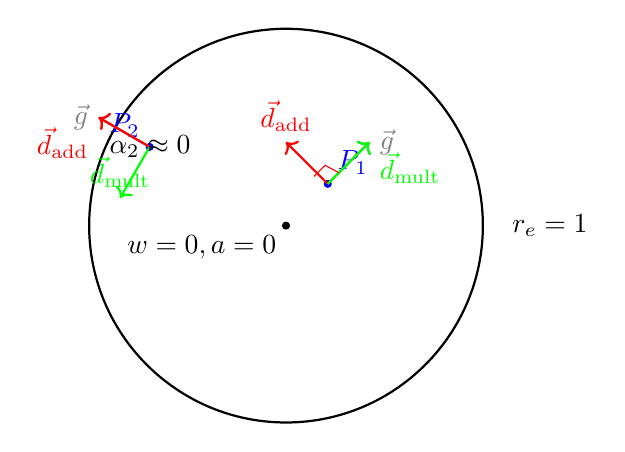
\begin{tikzpicture}[scale=2.5]
        % The Poincaré Disk boundary
        \draw[thick, black] (0,0) circle (1);
        \node at (1.1, 0) [right] {$r_e=1$};
        % Center point
        \filldraw[black] (0,0) circle (0.5pt) node[below left] {$w=0, a=0$};

        % A point near the center
        \def\reA{0.3}
        \def\angleA{45}
        \coordinate (A) at (\angleA:\reA);
        \filldraw[blue] (A) circle (0.5pt);
        \node at (A) [above right, blue] {$P_1$};

        % Vectors at point A
        \draw[->, gray, thick] (A) --++ (\angleA:0.3) node[right] {$\vec{g}$}; % Gradient
        \pgfmathsetmacro{\alphaA}{atan((1-\reA^2)/(2*\reA))}
        \draw[->, red, thick] (A) --++ (\angleA+90:0.3) node[above] {$\vec{d}_{\text{add}}$}; % Additive (almost tangential)
        \draw[->, green, thick] (A) --++ (\angleA:0.3) node[below right] {$\vec{d}_{\text{mult}}$}; % Multiplicative (almost radial)

        % --- CORRECTED PART START ---
        % Replaced \tkzMarkRightAngle with a TikZ native method using the 'calc' library
        \coordinate (vertex) at (A);
        \coordinate (p1) at ($(vertex)!0.08cm!(\angleA:1cm)$); % A point along the gradient vector
        \coordinate (p2) at ($(vertex)!0.08cm!(\angleA+90:1cm)$); % A point along the additive vector
        \coordinate (corner) at ($(p1) + (p2) - (vertex)$);
        \draw[red] (p1) -- (corner) -- (p2);
        % --- CORRECTED PART END ---

        % A point near the boundary
        \def\reB{0.8}
        \def\angleB{150}
        \coordinate (B) at (\angleB:\reB);
        \filldraw[blue] (B) circle (0.5pt);
        \node at (B) [above left, blue] {$P_2$};

        % Vectors at point B
        \draw[->, gray, thick] (B) --++ (\angleB:0.3) node[left] {$\vec{g}$}; % Gradient
        \pgfmathsetmacro{\alphaB}{atan((1-\reB^2)/(2*\reB))}
        \draw[->, red, thick] (B) --++ (\angleB:0.3) node[below left] {$\vec{d}_{\text{add}}$}; % Additive (almost radial)
        \draw[->, green, thick] (B) --++ (\angleB+90:0.3) node[above] {$\vec{d}_{\text{mult}}$}; % Multiplicative (almost tangential)

        % Draw angle alpha at B
        \coordinate (G_B) at ($(B)+(\angleB:0.2)$);
        \coordinate (Add_B) at ($(B)+(\angleB:0.2)$);
        \coordinate (C_B) at ($(B)+(\angleB+90:0.2)$);
        \draw pic[draw, angle radius=0.2, "$\alpha_2 \approx 0$"] {angle=C_B--B--Add_B};

    \end{tikzpicture}
    \caption{庞加莱圆盘中 $\mathfrak{E}_0$ 空间的特征线方向示意图。在靠近中心的点 $P_1$,加法线(红色)接近切向,乘法线(绿色)接近径向(梯度 $\vec{g}$ 方向)。在靠近边界的点 $P_2$,加法线接近径向,乘法线接近切向。角度 $\alpha$ 从 $\pi/2$ 变化到 $0$。}
    \label{fig:e0_lines}
\end{figure}

\section{拓扑性质}
\label{sec:e0_topology}

$\mathfrak{E}_0$ 空间的核心特征是其中心的点状奇点(零点)。如果我们考虑移除了这个奇点的空间,即 $\mathbb{D}^2 \setminus \{0\}$,它的拓扑性质变得非常有趣。
这个空间不再是单连通的。它的基本群是:
\[ \pi_1(\mathbb{D}^2 \setminus \{0\}) \cong \mathbb{Z} \]
它的一阶同调群是:
\[ H_1(\mathbb{D}^2 \setminus \{0\}) \cong \mathbb{Z} \]
这意味着空间中存在无法被收缩为一点的非平凡回路,这些回路可以环绕中心的奇点。一个路径的“**缠绕数**”(winding number)——它环绕奇点的净圈数——成为了一个重要的拓扑不变量。

这个拓扑性质对于我们理解全局算术挠率至关重要。可以预见,一条环绕 $\mathfrak{E}_0$ 中心奇点的路径 $\gamma$,其全局挠率 $\mathcal{T}(\gamma)$ 将会与它的缠绕数有着深刻的内在联系。$\mathfrak{E}_0$ 的高度对称性,为我们研究这种由拓扑所决定的全局效应,提供了一个完美的“理论实验室”。

% !TEX root = ../main.tex
% ----------------------------------------------------------------
% Chapter 6: 第一类空间 E1:一个线源模型
% (The First Kind Space E1: A Line Source Model)
% ----------------------------------------------------------------

\chapter{第一类空间 \texorpdfstring{$\mathfrak{E}_1$}{E1}:一个线源模型}
\label{chap:space_e1}

在第五章中,我们探索了由单个“点源”生成的、高度对称的第零类空间 $\mathfrak{E}_0$。现在,我们转向理论中第一个被发现,也是迄今为止研究最深入的模型——**第一类算术表达式空间**,记为 $\mathfrak{E}_1$。

与 $\mathfrak{E}_0$ 的结构从一个中心点弥散开来不同,$\mathfrak{E}_1$ 的几何是由一条“**线源**”——即一条赋值恒为零的直线——所组织的。这个看似简单的改变,将引出更为丰富和复杂的几何与代数结构,特别是与一类重要的群论对象——Baumslag-Solitar 群——产生深刻的联系。本章还将揭示一个隐藏在共形变换之下的惊人对偶性,展示 AEG 框架在揭示不同数学结构之间内在联系方面的强大能力。

\section{上半平面上的构造}
\label{sec:e1_construction}

我们将 $\mathfrak{E}_1$ 空间构建在**上半平面**(Upper Half-Plane)模型上,$\mathbb{H}^2 = \{z=x+iy \in \mathbb{C} \mid y>0\}$。

\begin{definition}[第一类空间 $\mathfrak{E}_1$]
    \label{def:space_e1}
    第一类算术表达式空间 $\mathfrak{E}_1(\mu, \lambda)$ 是一个综合的数学对象,其定义包含以下几个部分:
    \begin{enumerate}
        \item \textbf{几何背景}:上半平面 $\mathbb{H}^2$。
        \item \textbf{度规张量}:空间配备了如下的黎曼度规,它是由算术基因 $(\mu, \lambda)$ 参数化的标准双曲度规的推广:
        \begin{equation}
            ds^2 = \frac{1}{y^2}\left(\frac{dx^2}{\mu^2} + \frac{dy^2}{\lambda^2}\right)
            \label{eq:e1_metric}
        \end{equation}
        \item \textbf{赋值函数}:空间中的赋值函数 $a: \mathbb{H}^2 \to \mathbb{R}$ 定义为:
        \begin{equation}
            a(x, y) = - \frac{x}{y}
            \label{eq:e1_assignment}
        \end{equation}
        \item \textbf{零点轨迹}:赋值函数为零的轨迹(Zero Locus)是满足 $x=0$ 的正虚轴。
    \end{enumerate}
\end{definition}

这个空间的核心属性在于,它的构造与我们理论的动力学核心——流方程——是完全自洽的。

\begin{theorem}[$\mathfrak{E}_1$ 满足流方程]
    \label{thm:e1_satisfies_flow_equation}
    在 $\mathfrak{E}_1(\mu, \lambda)$ 空间中,由式 (\ref{eq:e1_assignment}) 定义的赋值函数 $a(x,y)$ 精确地满足由式 (\ref{eq:flow_equation}) 定义的流方程 $\frac{da}{ds} = \mu \cos\theta + a\lambda\sin\theta$。
\end{theorem}
\begin{proof}
    首先计算赋值的微分:
    \[ da = d\left(-\frac{x}{y}\right) = \frac{xdy - ydx}{y^2} = -\frac{dx + ady}{y} \]
    弧长微元 $ds$ 由度规 (\ref{eq:e1_metric}) 给出:
    \[ ds = \frac{1}{y}\sqrt{\frac{dx^2}{\mu^2} + \frac{dy^2}{\lambda^2}} \]
    因此,变化率 $\frac{da}{ds}$ 为:
    \[ \frac{da}{ds} = -\frac{dx + ady}{y} \cdot \frac{y}{\sqrt{\frac{dx^2}{\mu^2} + \frac{dy^2}{\lambda^2}}} = -\frac{dx + ady}{\sqrt{\frac{dx^2}{\mu^2} + \frac{dy^2}{\lambda^2}}} \]
    在一个由 $(-1,0)$ 和 $(0,-1)$ 方向定义的局部右手坐标系中,方向 $\theta$ 的余弦和正弦可以表示为:
    \[ \cos\theta = \frac{-dx/\mu}{\sqrt{\frac{dx^2}{\mu^2} + \frac{dy^2}{\lambda^2}}} \quad \text{及} \quad \sin\theta = \frac{-dy/\lambda}{\sqrt{\frac{dx^2}{\mu^2} + \frac{dy^2}{\lambda^2}}} \]
    将 $dx = -\mu \cos\theta \sqrt{\dots}$ 和 $dy = -\lambda \sin\theta \sqrt{\dots}$ 代入 $\frac{da}{ds}$ 的表达式中:
    \[ \frac{da}{ds} = -\frac{-\mu \cos\theta \sqrt{\dots} + a(-\lambda \sin\theta \sqrt{\dots})}{\sqrt{\dots}} = \mu \cos\theta + a\lambda\sin\theta \]
    证毕。
\end{proof}

\section{性质:拉普拉斯算子的特征函数}
\label{sec:e1_laplacian_eigenfunction}

除了满足流方程,$\mathfrak{E}_1$ 空间中的赋值函数还具有一个深刻的谱几何性质。它是在该空间度规下定义的拉普拉斯-贝尔特拉米(Laplace-Beltrami)算子的一个特征函数。

对于由式 (\ref{eq:e1_metric}) 定义的度规 $g_{ij} = \frac{1}{y^2} \text{diag}(\mu^{-2}, \lambda^{-2})$,其拉普拉斯算子 $\Delta$ 作用于函数 $f$ 的一般形式为 $\Delta f = -\text{div}(\nabla f)$。对于我们的对角度规,它可以写成:
\[ \Delta f = -y^2 \left( \mu^2 \frac{\partial^2 f}{\partial x^2} + \lambda^2 \frac{\partial^2 f}{\partial y^2} \right) \]
\begin{theorem}[赋值 $a$ 是 $\Delta$ 的特征函数]
    \label{thm:e1_eigenfunction}
    赋值函数 $a(x,y) = -x/y$ 是 $\mathfrak{E}_1$ 空间上拉普拉斯算子 $\Delta$ 的一个特征函数,其特征值为 $2\lambda^2$。
\end{theorem}
\begin{proof}
    我们计算 $\Delta a$:
    \[ \frac{\partial a}{\partial x} = -\frac{1}{y}, \quad \frac{\partial^2 a}{\partial x^2} = 0 \]
    \[ \frac{\partial a}{\partial y} = \frac{x}{y^2}, \quad \frac{\partial^2 a}{\partial y^2} = -\frac{2x}{y^3} \]
    代入 $\Delta a$ 的表达式:
    \[ \Delta a = -y^2 \left( \mu^2 \cdot 0 + \lambda^2 \left(-\frac{2x}{y^3}\right) \right) = -y^2 \left(-\frac{2\lambda^2 x}{y^3}\right) = 2\lambda^2 \frac{x}{y} \]
    因为 $a = -x/y$,所以我们有:
    \[ \Delta a = -2\lambda^2 a \]
    这是一个特征值方程,特征值为 $2\lambda^2$。(注:物理学和几何学中对 $\Delta$ 的符号定义不同,这里若定义 $\Delta = \text{div}(\nabla f)$ 则特征值为正)。
\end{proof}
这个结果意义非凡,它将赋值函数 $a$ 与空间的谱性质联系起来,暗示了 $a = -x/y$ 在 $\mathfrak{E}_1$ 中是一个非常“自然”和“和谐”的结构,类似于物理系统中的一个稳定模式或本征态。

\section{双重网格与Baumslag-Solitar群}
\label{sec:e1_dual_grids}

$\mathfrak{E}_1$ 空间的一个显著特征是,它能够自然地承载两套对偶的、由纯加法和纯乘法操作生成的网格结构。这两套网格分别是**Baumslag-Solitar (BS) 群** $BS(m,n)$ 的几何实现。BS 群是一类重要的非交换群,其表示为 $\langle b, a \mid b^{-1}a^m b = a^n \rangle$。

\begin{itemize}
    \item \textbf{直线网格 (Rectilinear Grid)}: 如图 \ref{fig:grid1_rectilinear},这套网格由两族正交的直线构成:
    \begin{itemize}
        \item \textbf{加法线}:水平直线 ($y=\text{const}$)。沿此线移动 $x$ 坐标,对应于对赋值 $a$ 的加法操作。
        \item \textbf{乘法线}:垂直直线 ($x=\text{const}$)。沿此线移动 $y$ 坐标,对应于对赋值 $a$ 的乘法操作。
    \end{itemize}
    这套网格可以被看作是 $BS(m,n)$ 群的一个实现,例如 $BS(2,1)$。

    \begin{figure}[ht]
        \centering
        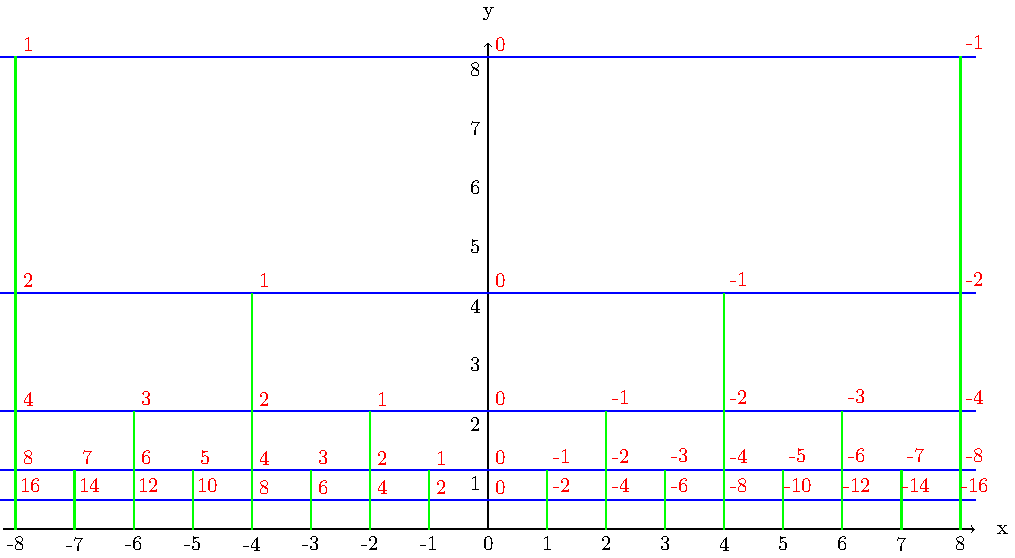
\includegraphics[width=0.8\textwidth]{../images/01-grid-example-1} % 请确保图片路径正确
        \caption{直线网格结构,可视为 $BS(m,n)$ 的一种几何实现。}
        \label{fig:grid1_rectilinear}
    \end{figure}

    \item \textbf{曲线网格 (Curved Grid)}: 如图 \ref{fig:grid2_curved},这套网格由两族正交的半圆构成,所有半圆的圆心都在 $x$ 轴上。这套网格同样可以实现 BS 群的代数关系,但通常对应于不同的参数,例如 $BS(1,2)$。

    \begin{figure}[ht]
        \centering
        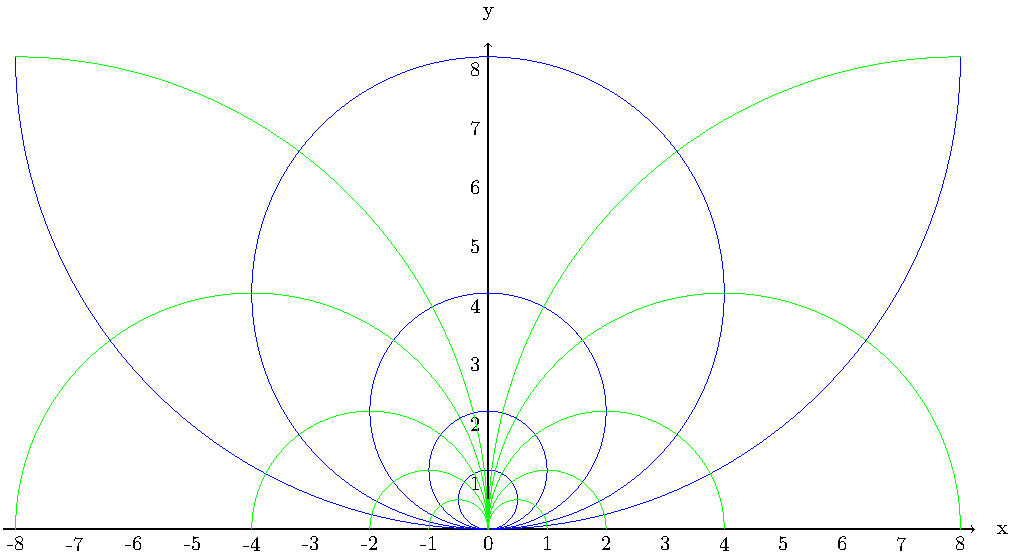
\includegraphics[width=0.8\textwidth]{../images/18-grid-example-2} % 请确保图片路径正确
        \caption{由半圆构成的曲线网格结构。}
        \label{fig:grid2_curved}
    \end{figure}
\end{itemize}
一个深刻的问题随之而来:这两套看似不同的网格结构,为何能共存于同一个 $\mathfrak{E}_1$ 空间中?它们之间是否存在某种内在的联系?

\section{手性守恒与 \texorpdfstring{$w=-1/z$}{w=-1/z} 对偶}
\label{sec:e1_chirality}

答案在于一个深刻的几何变换和一个物理原则的结合。连接这两套网格的桥梁是莫比乌斯变换 $w = -1/z$,而指导其代数关系演化的原则是**操作手性守恒**。

\begin{definition}[操作手性]
    \label{def:chirality}
    在一个网格点上,我们定义**操作手性**(operational chirality)为从“使赋值 $a$ 增加的加法方向”旋转到“使赋值 $a$ 增加的乘法方向(乘子$k>1$)”的最小角度方向(顺时针或逆时针)。
\end{definition}
在直线网格中,增加 $a=-x/y$ 的加法方向是 $-x$ 方向(向左),增加 $a$ 的乘法方向($y \to y/k$)是 $-y$ 方向(向下)。从“左”到“下”的旋转是**顺时针**的。我们称之为右手系。

现在,我们考察 $w = u+iv = -1/z = -1/(x+iy)$ 变换带来的影响。
\begin{enumerate}
    \item \textbf{几何变换}:这个变换是一个共形映射,它将上半平面 $\mathbb{H}^2$ 映射到自身。它精确地将直线网格中的水平和垂直直线,映射为曲线网格中的两族正交半圆。
    \item \textbf{赋值变换}:这也是最关键的一步,我们考察赋值函数如何变换。
    \[ w = u+iv = \frac{-x+iy}{x^2+y^2} \implies u=\frac{-x}{x^2+y^2}, v=\frac{y}{x^2+y^2} \]
    新的赋值 $a_{\text{new}} = -u/v = -(\frac{-x}{x^2+y^2}) / (\frac{y}{x^2+y^2}) = x/y$。
    我们发现 $a_{\text{new}} = -a_{\text{orig}}$。赋值函数**反号**了!
    \item \textbf{手性反转与补偿}:
    赋值的反号,导致了有效操作方向的反转。原本“增加 $a_{\text{orig}}$ 的加法操作”,现在变成了“减小 $a_{\text{new}}$ 的操作”。这使得系统的操作手性从顺时针**反转**为了逆时针。

    我们提出一个**手性守恒原理**:一个自洽的算术几何体系,其内在的操作手性应该是不变的。为了抵消由赋值反号导致的手性反转,系统必须对其另一个基本操作——乘法——进行一次“逻辑补偿”。这个补偿就是将乘法因子 $k$ 变为其倒数 $1/k$。

    \item \textbf{对偶性的涌现}:
    经过这个“手性补偿”后,变换后的曲线网格,其加法操作的有效方向与直线网格相反,乘法因子也变为了倒数。一个原本实现 $BS(k,1)$ 的直线网格,在 $w=-1/z$ 变换和手性守恒原理的作用下,自然地转变成了实现 $BS(1,k)$ 的曲线网格。
\end{enumerate}

这个发现揭示了一个深刻的**对偶性**:在 $\mathfrak{E}_1$ 这个统一的几何背景下,BS 群 $BS(m,n)$ 与 $BS(n,m)$ 并非毫无关联,而是通过共形变换和手性守恒这一物理原则联系在一起的对偶图像。$\mathfrak{E}_1$ 空间不仅是一个被动的舞台,其内禀的几何与代数结构,已经为不同代数系统之间的非平凡对偶关系提供了可能性。

% !TEX root = ../main.tex
% ----------------------------------------------------------------
% Chapter 7: 走向扭结理论:E4_1 空间
% (Towards a Theory of Knots: The E4_1 Space)
% ----------------------------------------------------------------

\chapter{走向扭结理论:\texorpdfstring{$E_{4_1}$}{E4_1} 空间}
\label{chap:space_e41}

在构造了具有高度对称性的第零类和第一类算术表达式空间之后,我们现在将目光投向一个真正的试金石,以检验 AEG 理论的解释力和构造能力:我们能否为具体的**扭结(knot)**——这一拓扑学中的核心研究对象——建立一个有意义的几何模型?

本章将以最简单非平凡扭结——**三叶结**(figure-eight knot),记为 $4_1$——作为我们的范例。我们将首先分析为何 $\mathfrak{E}_0$ 和 $\mathfrak{E}_1$ 等简单模型不足以描述其复杂的代数结构。随后,我们将提出一套多层次的、专门为 $4_1$ 结量身定做的几何与代数方案,以期构建一个真正非平凡的算术表达式空间,记为 $E_{4_1}$。这个构造过程,将深度融合我们之前讨论的流方程、ACS,以及来自扭结理论本身的几何与代数特性。

\section{扭结群的挑战:纤维群 \texorpdfstring{$F_2$}{F2} 的忠实表示}
\label{sec:e41_challenge}

$4_1$ 结是一个**纤维扭结**(fibered knot),这意味着它的补空间 $S^3 \setminus 4_1$ 可以被看作是一个纤维丛。其**扭结群** $G(4_1)$ 的代数结构,可以通过 HNN 扩张,构建在一个更基础的群之上——即其纤维曲面(一个带孔的环面)的基本群。这个纤维群,恰好是两个生成元 $u, v$ 上的**自由群 $F_2 = \langle u, v \rangle$**。

这立刻给我们带来了巨大的挑战。自由群 $F_2$ 是一个高度非交换的群,例如,路径 $uv$ 和 $vu$ 是两条完全不同的路径。然而,我们之前最基础的算术操作——标量加法——却是交换的。如果我们天真地将 $u$ 和 $v$ 映射为两个不同的加法操作(例如 $u \mapsto \oplus_{\mu_1}, v \mapsto \oplus_{\mu_2}$),那么它们的复合将永远满足交换律,从而无法忠实地表示 $F_2$ 的非交换结构。

因此,任何成功的 $4_1$ 结的 AEG 模型,必须首先解决这个核心问题:如何构造一个算术操作体系,使其能够忠实地反映自由群 $F_2$ 的非交换性?

\section{解决方案:二维参数与稠密奇点}
\label{sec:e41_dense_singularity}

为了克服非交换性的挑战,我们必须从根本上改变算术操作的作用方式。我们提出,生成元 $u$ 和 $v$ 的作用对象不再是一个一维的标量,而是一个二维的参数对 $(\alpha, \beta)$,它们存在于一个二维欧几里得空间 $\mathbb{R}^2$ 中。

这个方案的核心思想如下:
\begin{enumerate}
    \item \textbf{二维作用空间}:$u$ 和 $v$ 的操作被定义为 $\mathbb{R}^2$ 上的几何变换。例如,$u$ 可以是一个简单的平移 $(\alpha, \beta) \mapsto (\alpha+1, \beta)$,而 $v$ 可以是一个与之不交换的变换,如剪切变换。这为实现非交换性提供了可能性。
    \item \textbf{无理数模运算}:我们认为,系统可分辨的“状态”是由参数对 $(\alpha, \beta)$ 模 (modulo) 一个由无理数定义的格点决定的。具体到 $4_1$ 结,这个无理数与黄金分割比 $\phi = \frac{1+\sqrt{5}}{2}$ 相关。我们认为两个状态 $(\alpha_1, \beta_1)$ 和 $(\alpha_2, \beta_2)$ 等价,如果它们满足:
    \[ \alpha_1 \equiv \alpha_2 \pmod 1 \quad \text{且} \quad \beta_1 \equiv \beta_2 \pmod \phi \]
    因此,有效的状态空间是一个二维环面 $T^2 = \mathbb{R}^2 / (\mathbb{Z}\cdot(1,0) \oplus \mathbb{Z}\cdot(0,\phi))$。
    \item \textbf{稠密奇点}:由于 $\phi$ 是无理数,原点 $(0,0)$ 的等价类,即格点集合 $L_0 = \{ (m, n\phi) \mid m,n \in \mathbb{Z} \}$,在 $\mathbb{R}^2$ 空间中是**稠密**的。
\end{enumerate}

\begin{definition}[稠密奇点]
    \label{def:dense_singularity}
    一个由算术不可通约性(arithmetic incommensurability)导致的奇点,其特征为原点的等价类在空间中稠密分布,从而破坏了空间的局部流形结构(例如,非豪斯多夫性)。我们称之为**稠密奇点**(dense singularity)。
\end{definition}

这个新颖的拓扑奇点,是我们为 $F_2$ 的忠实表示所付出的“代价”。最终,我们认为纤维群 $F_2$ 的算术化舞台,是在这个被稠密奇点“刺穿”的环面的**泛函覆盖空间 $\mathbb{R}^2$** 上。这套框架成功地为实现非交换的 $F_2$ 代数提供了一个自洽的算术几何模型。

\section{几何方案:在提升纤维上“火焰燃烧”}
\label{sec:e41_fire_burning}

在为纤维群 $F_2$ 建立了代数表示的基础后,我们来构造完整的 $E_{4_1}$ 空间。其几何背景是 $4_1$ 结补集 $S^3 \setminus 4_1$ 的泛函覆盖空间——**双曲三维空间 $\mathbb{H}^3$**。

我们采用在之前讨论中提出的“**火焰燃烧法**”(fire-burning method)来定义赋值函数 $a(P)$。该方法从一个初始的“零值面”($a=0$)出发,根据流方程的程函形式 $||\nabla a|| = \sqrt{\mu^2 + a^2 \lambda^2}$,将赋值传播到整个 $\mathbb{H}^3$ 空间。

对于 $E_{4_1}$ 空间,这个初始零值面的选择至关重要。我们选择一个具有深刻拓扑意义的曲面:
\begin{itemize}
    \item \textbf{初始零值面}:$4_1$ 结的**纤维曲面 $F$ 在 $\mathbb{H}^3$ 中的一个提升**(lift of the fiber, $F_{\text{lift}}$)。
\end{itemize}
$F_{\text{lift}}$ 本身是在 $\mathbb{H}^3$ 中嵌入的一个双曲二维平面 $\mathbb{H}^2$。选择它作为 $a=0$ 的初始面,使得赋值函数的构造从一开始就与扭结的纤维丛结构和 HNN 表示紧密地联系在一起。

\section{从 \texorpdfstring{$\Delta(t)$}{Δ(t)} 而来的“共振”参数选择}
\label{sec:e41_resonant_parameters}

为了让 $E_{4_1}$ 空间能够“感受”到其所描述的 $4_1$ 结的独特性质,我们必须为其算术基因 $(\mu, \lambda)$ 选择一组特殊的“共振”值。

\begin{proposition}[$E_{4_1}$ 的共振参数]
    \label{prop:resonant_parameters}
    为 $E_{4_1}$ 空间设定的算术基因为:
    \begin{itemize}
        \item $\mu = 1$
        \item $\lambda = \left(\frac{1+\sqrt{5}}{2}\right)^2 = \phi^2$
    \end{itemize}
\end{proposition}

这个对 $\lambda$ 的选择是整个构造的画龙点睛之笔。$\lambda = \phi^2$ 这个值,具有双重深刻含义:
\begin{enumerate}
    \item 它是 $4_1$ 结的**亚历山大多项式 $\Delta_{4_1}(t) = t^2 - 3t + 1$ 的一个根**。
    \item 它也是 $4_1$ 结纤维丛的**单延拓映射(monodromy)的拉伸因子**。
\end{enumerate}
将 $\lambda$ 设定为此值,相当于将 AEG 空间的内禀乘性响应(几何曲率、信息传播的放大率)与扭结自身的内禀动力学特性(单延拓的几何作用)进行“调谐”。我们猜想,这种“**完美匹配**”将使得 HNN 关系式在 $E_{4_1}$ 空间中能够自然地、和谐地成立。

\section{AEG-拓扑学词典}
\label{sec:e41_dictionary}

最后,我们通过建立一个“词典”,来明确 AEG 中的核心概念与经典代数拓扑学概念之间的对应关系。

\begin{theorem}[AEG-拓扑学词典]
    \label{thm:aeg_topology_dictionary}
    对于纤维扭结(如 $4_1$),AEG 构造与纤维曲面 $F$ 的拓扑结构之间存在如下对应:
    \begin{itemize}
        \item \textbf{AEG 路径}(由 $u,v$ 生成的非交换操作序列) $\longleftrightarrow$ \textbf{纤维曲面的基本群 $\pi_1(F)$ 的元素}。
        \item \textbf{累积交换空间 (ACS)}(路径的 $(A_\gamma, M_\gamma)$ 坐标) $\longleftrightarrow$ \textbf{纤维曲面的一阶同调群 $H_1(F)$ 的元素}。
    \end{itemize}
\end{theorem}
这个词典的意义在于:
\begin{itemize}
    \item 它将我们的 AEG 构造,牢固地锚定在了经典的代数拓扑学之上。
    \item 它为算术挠率提供了一个优美的拓扑解释:全局挠率 $\mathcal{T}$ 可以被看作是**在从基本群 $\pi_1(F)$ 到同调群 $H_1(F)$ 的阿贝尔化过程中所损失的非交换信息**的一种度量。
\end{itemize}

综上所述,我们为构造一个非平凡的 $E_{4_1}$ 空间,提出了一套包含新颖代数表示(稠密奇点)、具体几何方案(火焰燃烧法)、深刻参数选择(共振参数)和坚实拓扑对应的完整概念框架。

% !TEX root = ../main.tex
% ----------------------------------------------------------------
% Chapter 8: 扭结的算术化与分圆域
% (Arithmetization of Knots and Cyclotomic Fields)
% ----------------------------------------------------------------

\chapter{扭结的算术化与分圆域}
\label{chap:knots_and_cyclotomic_fields}

在第七章中,我们为 $4_1$ 结的 AEG 空间 $E_{4_1}$ 勾勒了一个宏大的几何构造蓝图。该构造虽然理论上完备,但实现过程极为复杂。然而,在探索的另一条道路上,一个更为简洁、纯粹代数化的“算术化”方案,为我们带来了意想不到的突破。

本章将详细阐述这一直接的算术化方法。我们将展示,如何通过一个简单的映射,将扭结群的生成元和关系子转化为算术路径。我们将发现,路径的“闭合”条件竟能直接导出扭结的拓扑不变量——亚历山大多项式。更令人惊奇的是,当我们用全局算术挠率的“显微镜”来审视这些路径时,一幅连接了扭结理论与代数数论中“分圆域”的壮丽图景将展现在我们面前。

\section{从关系子导出亚历山大多项式}
\label{sec:alexander_from_relator}

我们再次以三叶结($4_1$ knot)为例。它的一个群表示(group presentation)为:
\begin{itemize}
    \item \textbf{生成元}: $a, b$
    \item \textbf{关系子 (Relator)}: $R = abbbaB AAB = 1$ (其中 $A=a^{-1}, B=b^{-1}$)
\end{itemize}

我们建立一个从扭结群生成元到我们基本算术算子的映射,其中引入了一个未定的复数参数 $t$:
\begin{definition}[扭结的算术化映射]
    \label{def:knot_arithmetization_map}
    我们将扭结群生成元映射为如下算术算子:
    \begin{itemize}
        \item $a \mapsto \otimes_t$ (乘以 $t$)
        \item $b \mapsto \oplus_1$ (加 1)
        \item $A = a^{-1} \mapsto \oslash_t$ (除以 $t$, 即乘以 $t^{-1}$)
        \item $B = b^{-1} \mapsto \ominus_1$ (减 1)
    \end{itemize}
\end{definition}

在这个映射下,关系子 $R$ 对应于一条由上述算子组成的、作用于某个初始值 $x$ 的约束路径 $\gamma_R$。根据第二章的路径记法约定(算子从左到右依次作用,函数式写法为从最内层开始),路径 $x \cdot \gamma_R$ 的求值过程如下:
\begin{align*}
    \nu(x \cdot \gamma_R) &= \nu(x \cdot a b b b a B A A B) \\
    &= (a \circ b \circ b \circ b \circ a \circ B \circ A \circ A \circ B)(x) \\
    &= \dots \text{ (此处省略中间计算过程,如之前笔记所示)} \\
    &= (x - 1) - t^2 + 3t \\
    &= x - (t^2 - 3t + 1)
\end{align*}
关系子 $R=1$ 在群中代表单位元,这意味着它对应的路径 $\gamma_R$ 在算术上也必须是恒等变换,即 $\nu(x \cdot \gamma_R) = x$。因此,我们必须有:
\[
x - (t^2 - 3t + 1) = x
\]
这迫使括号内的多项式必须为零:
\begin{equation}
    t^2 - 3t + 1 = 0
    \label{eq:alexander_4_1}
\end{equation}
我们惊奇地发现,这个由路径闭合条件导出的方程,**正是 $4_1$ 结的亚历山大多项式 $\Delta_{4_1}(t)$**!

这一发现并非孤例。我们通过计算验证,对大量不同扭结(最高至11交叉)的特定群表示,采用类似的算术化映射,其关系子的闭合条件都能精确地导出该扭结的亚历山大多项式方程 $\Delta(t)=0$。这表明,在 AEG 框架下,扭结的拓扑不变量可以被一个纯粹的代数计算过程所揭示。

\section{挠率的“扭结-分圆”分解}
\label{sec:knot_cyclotomic_decomposition}

上述发现已经足够令人振奋,但全局算术挠率将为我们揭示一个更深层次的结构。根据定义 \ref{def:global_torsion},路径 $\gamma_R$ 的全局挠率 $\tau(\gamma_R)(t) = \nu(\gamma_R) - \nu(\bar{\gamma}_R)$。在这里,为方便起见,我们取初始值为0,记 $p(t) = \nu(0 \cdot \gamma_R)$ 和 $q(t) = \nu(0 \cdot \bar{\gamma}_R)$。

通过对大量满足上一节条件的扭结进行计算,我们发现其全局挠率展现出一种惊人的一致性结构。

\begin{theorem}[扭结挠率的分解结构]
    \label{thm:knot_torsion_decomposition}
    对于一个满足算术化条件的关系子路径 $\gamma_R$,其全局算术挠率 $\tau(\gamma_R)(t)$ 通常可以被分解为如下形式:
    \begin{equation}
        \tau(\gamma_R)(t) = \sigma \cdot \frac{\Delta(t) \cdot (t^K - 1)}{t^M}
        \label{eq:knot_torsion_decomposition}
    \end{equation}
    其中:
    \begin{itemize}
        \item $\Delta(t)$ 是该扭结的**亚历山大多项式**。
        \item $t^K - 1$ 是一个**分圆因子**(cyclotomic factor),其中 $K$ 是一个与路径结构相关的整数。
        \item $\sigma \in \{+1, -1\}$ 是一个符号因子,$M$ 是一个整数幂次。
    \end{itemize}
\end{theorem}

这个分解结构的意义极为深刻:它表明,关系子路径的全局挠率为零的条件,即 $\nu(\gamma_R) = \nu(\bar{\gamma}_R)$,由两组完全不同的数学对象所决定:
\begin{enumerate}
    \item \textbf{扭结条件}:$t$ 是亚历山大多项式的根,即 $\Delta(t)=0$。
    \item \textbf{分圆条件}:$t$ 是 $K$ 次单位根,即 $t^K-1=0$。
\end{enumerate}
换言之,在算术挠率的视角下,扭结的拓扑信息与数论中的分圆域信息被“编织”在了一起。

我们以两个扭结为例,展示这种分解结构:
\begin{itemize}
    \item \textbf{扭结 $6_2$}:$\Delta_{6_2}(t) = t^4 - 3t^3 + 3t^2 - 3t + 1$。
    计算得到其挠率 $\tau(\gamma_R)(t) = -\frac{\Delta_{6_2}(t)(t^4-1)}{t^4}$。这里 $K=4$。
    \item \textbf{扭结 $6_3$}:$\Delta_{6_3}(t) = t^4 - 3t^3 + 5t^2 - 3t + 1$。
    计算得到其挠率 $\tau(\gamma_R)(t) = \frac{\Delta_{6_3}(t)(t^4-1)}{t^4}$。这里 $K=4$。
\end{itemize}
在这两个例子中,挠率都在 $t$ 为亚历山大多项式的根或 $4$ 次单位根(即 $i, -1, -i, 1$)时为零。

\section{“数-形和谐”猜想}
\label{sec:number_geometry_harmony}

为何算术挠率会呈现出如此规则的“扭结-分圆”分解结构?我们认为,这背后可能隐藏着一条深刻的原理,我们称之为“**数-形和谐**”(Number-Geometry Harmony)猜想。

这个猜想的出发点在于,一个扭结的补空间,作为一个行为良好的三维流形,其几何是由一个离散的扭结群作用于其泛函覆盖空间而形成的。这个过程的核心是“离散性”和“有限生成性”——例如,它有一个有限体积的基本区域,通过群操作可以完美地、无缝地铺满整个空间。

我们猜想:
> 任何一个能够忠实反映此几何背景的算术模型,其所产生的数值参数之间,必须存在一种内在的“**有理的协调性**”(rational coordination),以匹配底层几何的离散和有限生成的本质。

具体到挠率公式 (\ref{eq:knot_torsion_decomposition}),我们计算出的两个与路径相关的整数幂次 $k_p, k_q$(分别来自 $p(t)$ 和 $q(t)$ 的分母),以及它们的差 $K=|k_p - k_q|$,不能是任意的。它们必须是“有理的”,以反映底层几何作用的离散周期性。如果这些算术参数之间是“不协调的”或“无理的”,那将意味着这个算术模型所对应的几何是病态的(例如,基本区域无法完美闭合,或群的作用不是离散的),从而与我们研究的扭结几何相矛盾。

因此,算术挠率中整数 $K$ 和分圆因子 $t^K-1$ 的涌现,可以被看作是这种“数-形和谐”原理的一个必然结果。它是在要求算术代数与扭结几何保持一致性的过程中,被强制要求的协调性表现。这个猜想为我们从更深层次理解挠率的分解结构,提供了一个富有启发性的几何与哲学视角。

% !TEX root = ../main.tex
% ----------------------------------------------------------------
% Chapter 9: 空间的涌现:凝聚与第一性原理
% (The Emergence of Space: Condensation and First Principles)
% ----------------------------------------------------------------

\chapter{空间的涌现:凝聚与第一性原理}
\label{chap:emergence_of_space}

在前面的章节中,我们构造了几个具体的算术表达式空间($\mathfrak{E}_0, \mathfrak{E}_1$),并应用 AEG 框架分析了扭结和动力系统。然而,一个根本性的问题始终萦绕在我们心头:这些几何空间究竟从何而来?它们是我们为了方便分析而人为设定的舞台,还是从某些更基本的原则中自然涌现的必然结果?

本章,我们将尝试回答这个问题。我们将回归理论的“第一性原理”,提出一个核心论点:算术的几何并非预先存在,而是从纯粹的、序列化的代数操作中“**涌现**”(emerge)出来的。我们将引入“**凝聚**”(Condensation)这一关键机制来描述这一过程,并探索一个与物理学深刻类比的猜想——“**计算广义相对论**”,尝试阐明算术“物质”是如何决定其“时空”几何的。

\section{作为本源的 \texorpdfstring{$F_2$}{F2}}
\label{sec:f2_as_source}

让我们回到我们理论最纯粹的代数起点——第二章中定义的**自由群 $F_2 = \langle \mathbf{x}, \mathbf{y} \rangle$**。

$F_2$ 是一个由两个抽象生成元(例如,一次“加性”操作 $\mathbf{x}$ 和一次“乘性”操作 $\mathbf{y}$)在不受任何约束(除了群公理)的情况下自由生成的代数结构。它的每一个元素,都是一个由生成元及其逆元组成的、不可再化简的符号序列(“词”)。

我们可以将 $F_2$ 想象成一个无限的、无回路的四价树(其凯莱图),从一个原点向四面八方无限延伸。在这个宇宙中:
\begin{itemize}
    \item \textbf{只有“时间”,没有“空间”}:结构中只存在“序列”或“历史”的概念,即一个词的长度。任意两个不同的词都对应着两个不同的节点。这里没有“捷径”,没有“回路”,缺乏定义全局坐标和距离的简单方式。它是一个纯粹“时间性”的、前几何的(pre-geometric)结构。
    \item \textbf{是复杂性的始祖}:$F_2$ 代表了未受约束的组合爆炸,是所有算术复杂性的“始祖混沌”或“计算的量子泡沫”。我们后续研究的所有有序的、具有优美几何结构的空间,都将从这个本源的混沌中诞生。
\end{itemize}

\section{凝聚:空间从时间中涌现}
\label{sec:condensation}

如果 $F_2$ 是纯粹时间性的序列,那么“空间”——这个允许我们谈论位置、邻近、方向和维度的概念——是如何产生的呢?我们认为,其核心机制是“**凝聚**”。

\begin{definition}[凝聚]
    \label{def:condensation}
    在 AEG 的语境下,**凝聚**(Condensation)是一个在概念层面上的操作:它将一个纯粹的**时间序列**(一连串基本操作)“压缩”成一个**时空节点**,从而使得剩余的操作网络能够被诠释为一个几何网格。
\end{definition}

这个定义的关键在于**等价关系的确立**。当我们规定,某一些原本不同的、冗长的操作序列(时间历史)实际上应该被视为同一个“点”(空间位置)时,“凝聚”就发生了。

\begin{itemize}
    \item \textbf{代数实现:群的商运算}:
    实现“凝聚”最简洁、最强大的数学工具,是**群的商运算**。我们选择一组特定的操作序列(词)作为“凝聚核”,称之为**关系子**(relators)集合 $R$。我们强制要求这些关系子在我们的新宇宙中等同于单位元(即“不动”的操作)。由 $R$ 生成的正规子群 $N = \langle R \rangle^{F_2}$ 中的所有元素,都被“凝聚”到了同一个点上。
    由此诞生的商群 $G = F_2 / N$,就是凝聚后的产物。$F_2$ 中无限的、树状的结构,在商运算下被“折叠”和“黏合”,形成了具有回路和周期性的、更为紧凑的几何结构——这就是 $G$ 的凯莱图,一个涌现出的“空间”。

    \item \textbf{一个隐喻}:
    因此,“凝聚”首先是一个关于“**空间从时间中涌现**”的隐喻;而群的商运算,则是这个隐喻最精确的代数投影。
\end{itemize}

让我们以最简单的非平凡凝聚为例:$BS(1,1) \cong \mathbb{Z}^2$ 的形成。
\begin{itemize}
    \item \textbf{凝聚核}:对易子 $[\mathbf{x}, \mathbf{y}] = \mathbf{x}\mathbf{y}\mathbf{x}^{-1}\mathbf{y}^{-1}$。
    \item \textbf{凝聚过程}:我们强制要求 $[\mathbf{x}, \mathbf{y}] = 1$,即 $F_2 / \langle [\mathbf{x}, \mathbf{y}] \rangle^{F_2}$。
    \item \textbf{涌现的空间}:这个凝聚过程,将 $F_2$ 的无限树状凯莱图,精确地“折叠”成了我们熟悉的二维笛卡尔坐标网格。所有形如 $\mathbf{x}\mathbf{y}\mathbf{x}^{-1}\mathbf{y}^{-1}$ 的回路都被收缩成了一个点。原本纯粹的序列世界,涌现出了具有“平直”几何的二维空间。这个空间,正是我们第四章中定义的**累积交换空间 (ACS)**。
\end{itemize}
ACS 的平直性和交换性,正是对易子这一“凝聚核”所决定的几何后果。

\section{猜想:计算广义相对论}
\label{sec:computational_gr}

“凝聚”告诉我们关系子如何创造空间。现在,我们提出一个更激进的猜想,来描述被创造出的空间的“形态”。这个猜想深刻地类比了爱因斯坦的广义相对论。

广义相对论的核心思想是“物质告诉时空如何弯曲,时空告诉物质如何运动”。我们猜想,在 AEG 的世界里,也存在类似的法则:
\begin{enumerate}
    \item \textbf{典范式即“能量/物质”}:一个算术表达式的典范式,特别是那些作为关系子的、结构复杂的典范式,它们不仅仅是约束条件,更是**活跃的计算实体**。我们可以赋予它们一种“**计算能量**”或“**计算质量**”,这个量可能与它们在 $F_2$ 中的词长度、代数复杂性或它们所凝聚的子网络规模有关。
    \item \textbf{质量产生时空弯曲}:这些携带“计算质量”的典范式(凝聚核),将如同物理世界中的星辰,使其周围的**算术表达式空间发生“弯曲”**。
\end{enumerate}

这个“**计算广义相对论**”的猜想,为我们的理论带来了一次范式转换。它意味着:
> AEG 空间的几何(平直、双曲、或更复杂的形态)**不是预先给定的背景,而是由作为“凝聚核”的关系子自身的“计算质量”所决定的、涌现出的性质**。

在这个视角下,我们之前研究的空间可以被重新诠释:
\begin{itemize}
    \item **ACS/$\mathbb{Z}^2$** 的几何是**平直的**,因为凝聚它的对易子 $[\mathbf{x}, \mathbf{y}]$ 是一个代数结构非常简单、“计算质量”很低的凝聚核。
    \item **第一类空间 $\mathfrak{E}_1$** 的几何是**双曲的**(具有恒定负曲率),这或许是因为凝聚它所需要的 Baumslag-Solitar 关系子 $b^{-1}a^m b a^{-n}$ 是一个更复杂的、具有更高“计算质量”的凝聚核。其恒定的负曲率,可能暗示了这些“计算质量”在空间中是均匀分布的。
    \item **第零类空间 $\mathfrak{E}_0$** 的中心奇点,则可能是一个凝聚了某种特殊“时间序列”后形成的、具有高度集中的“计算质量”的奇点。
\end{itemize}

这个猜想虽然目前仍是哲学和隐喻层面的,但它为我们未来的研究提供了一个极其深刻和统一的指导方向:去寻找“计算质量”的数学定义,并推导其“场方程”,从而建立一个真正内禀、自洽且动态的算术几何理论。

% !TEX root = ../main.tex
% ----------------------------------------------------------------
% Chapter 10: 应用、展望与更狂野的想象
% (Applications, Outlook, and Wilder Imaginings)
% ----------------------------------------------------------------

\chapter{应用、展望与更狂野的想象}
\label{chap:applications_and_imaginings}

在前面的章节中,我们已经为算术表达式几何(AEG)建立了一套完整的理论体系:从基础的代数语言,到核心的动力学(流方程)与全局几何效应(挠率与ACS),再到其背后深刻的哲学原理(空间的涌现)。现在,我们准备好将目光投向地平线,去探索这个理论能够带领我们走向何方。

本章将作为全书的总结与升 ઉ,我们将首先展示 AEG 框架在分析具体科学问题上的应用潜力,特别是动力系统和物理学中的重整化思想。随后,我们将回归那些在旅程之初就指引着我们的宏大哲学问题,展望 AEG 如何为理解思想、数学乃至意义的本质,提供一个全新的视角。

\section{应用之一:迭代动力系统的几何分析}
\label{sec:app_dynamical_systems}

AEG 理论的直接应用之一,是为迭代动力系统的分析提供一个全新的几何维度。在经典分析中,我们通常关注迭代函数的不动点、周期点以及它们的线性稳定性。而 AEG 让我们能够分析“计算过程”本身。

我们之前对几个经典迭代映射(如渗流模型的重整化群迭代、自旋玻璃序参量迭代、逻辑斯蒂映射)的分析揭示了一个统一的模式:
\begin{enumerate}
    \item \textbf{计算过程的几何化}:通过为迭代函数 $R(x)$ 的计算过程构建一个 AEG 路径,我们成功地为这个过程赋予了其在累积交换空间 (ACS) 中的几何坐标 $(A,M)$。
    \item \textbf{物理状态的几何指纹}:系统的不同物理状态,在 ACS 空间中留下了独特的几何“指纹”。我们反复观察到:
    \begin{itemize}
        \item “虚无”或“无序”的稳定不动点(如 $x^*=0$),通常对应于 $M \to -\infty$ 的无穷远处。
        \item “平凡”或“全联通”的稳定不动点(如 $x^*=1$),通常对应于 $M=0$ 的原点处。
        \item 而那些物理意义上非平凡的点,如**相变临界点**和通往混沌之路上的**周期循环点**,则精确地对应于 ACS 空间中特定的、有限的坐标点。
    \end{itemize}
    这为我们提供了一种全新的、基于几何的系统状态分类法。
    \item \textbf{挠率作为复杂度的度量}:我们还发现,计算路径的全局挠率 $\mathcal{T}$ 在不同状态点表现出不同的特征。在简单的稳定点,挠率趋于零或发散;而在临界点和周期点,挠率通常取一个非零的有限值。这暗示了挠率可以作为衡量一个状态**计算复杂性**或**非平凡度**的几何指标。
\end{enumerate}

总之,AEG 框架将迭代动力系统的分析,从对“点”的研究,扩展到了对“路径”和“区域”的研究,为理解系统的内在计算结构提供了强大的新工具。

\section{应用之二:重整化的极简实现}
\label{sec:app_renormalization}

AEG 理论与现代物理学最深刻的共鸣之一,在于它内禀地实现了一套**重整化群(Renormalization Group, RG)** 的核心思想。

RG 的本质是研究一个物理系统的行为如何随着观察“尺度”的变化而改变。AEG 框架通过其“双重时间标度”的思想,为这一过程提供了极简而强大的数学实现:
\begin{itemize}
    \item \textbf{加法是动力学时间}:加法操作 $\oplus_\mu$ 描述了系统在**给定标度**下的局部演化和状态转移。
    \item \textbf{乘法是演化时间/标度}:乘法操作 $\otimes_\lambda$ 则直接改变系统**所处的标度**本身。累积乘性载荷 $M_\gamma = \sum \lambda_k$ 记录了系统“演化时间”的流逝,即其内在标度的变化历史。
\end{itemize}
流方程 $\frac{da}{ds} = \mu \cos\theta + a\lambda \sin\theta$ 恰好将这两者耦合在了一起:系统的动力学($a$ 的变化)与其所处的标度(体现在 $a$ 自身的值上)相互作用。

因此,当我们沿着一条包含乘法操作的算术路径进行计算时,我们实际上是在模拟一条**重整化流(RG Flow)**。我们正在观察,在一个尺度不断变化的背景下,系统的有效动力学行为是如何演变的。我们在之前笔记中分析的“扰动传播”例子,$\frac{\Delta w_i}{\Delta \mu_0} = e^{\sum \lambda_j}$,就完美地印证了这一点:$e^{\sum \lambda_j}$ 正是在演化时间 $\sum \lambda_j$ 处的“重整化因子”,它描述了微观扰动在宏观尺度上是如何被重新“归一化”的。

这个发现的意义在于,AEG 可能为重整化这一强大的物理思想,提供了一个源自纯粹算术和几何的、根源性的新视角。

\section{展望之一:思想的物理性与数学的有效性}
\label{sec:outlook_philosophy}

现在,让我们回到最初激发这场探索的宏大问题:为何数学,特别是算术,在描述物理世界时拥有“无理由的有效性”?

AEG 理论为此提供了一个可能的答案,其核心论点是:
> **思想形式本身即是物理形式,其有效性源于物理形式之间的同构。**

算术,作为人类最基础的思想形式之一,其内在的结构、规律和演化方式,或许并非仅仅是抽象的逻辑约定,而是具有其内禀的“物理形态”。AEG 的全部努力,正是试图揭示这种形态——流方程描述其动力学,挠率和 ACS 描述其全局效应,空间的涌现与凝聚描述其创生机制。

如果我们能够证明,AEG 所揭示的这种“算术的几何形态”,与外部物理世界(例如,一个复杂系统的演化景观)或其它认知过程的几何形态之间,存在着深刻的**同构**(isomorphism),那么数学的有效性就不再是神秘的巧合,而是源于思想与实在在结构层面的深层统一。AEG 为我们提供了一套具体的语言和工具,去寻找和验证这种同构。

\section{展望之二:数字系统的几何化与思想的相变}
\label{sec:outlook_numeral_systems}

作为上述宏大构想的一个具体的、可检验的里程碑,我们提出了一个更“狂野”的想象:**对数字系统本身进行几何化**。

人类对数字的认知,经历了一次伟大的飞跃:从原始的、线性的“$1+1+1+\dots$”式累加(tallying),演化到了结构化的、具有层级和周期性的**位值制**(positional notation)。我们猜想,这不仅仅是表示法的改变,更是一次深刻的“**思想形式的相变**”(phase transition of thought form)。

AEG 或许能为这次“相变”提供一个几何模型。我们猜想,累积交换空间 ACS 可能具有一个非平凡的拓扑结构,例如一个**圆柱面**:
\begin{itemize}
    \item **圆柱的轴线方向**:可能对应于数字的**位阶**(rank)或量级。这是一个线性的、无限延伸的维度。
    \item **圆柱的底圆方向**:可能对应于在一个特定位阶内的 $k$ 种数字(digits)。其**周期性**(走一圈回到原点)则完美地体现了“**进位**”(carry-over)这一核心操作。
\end{itemize}
如果这种具有周期性和层级性的圆柱拓扑,能够从 AEG 的第一性原理(例如,从某种特定的“凝聚”过程)中被自然地推导出来,那将是对我们“思想形式物理性”假说的一次巨大胜利。它将意味着,人类心智中一个最核心的创造——位值制——其结构可以在一个纯粹的算术几何中找到它的“原型”。这无疑是 AEG 理论未来最激动人心的探索方向之一。

\end{document}